\chapter{Production d'ondes de matière}
\label{ch:BEC_manip}
%\begin{tikzpicture}[remember picture, overlay]
%\node[anchor=north east,inner sep=0pt] at (current page.north east) {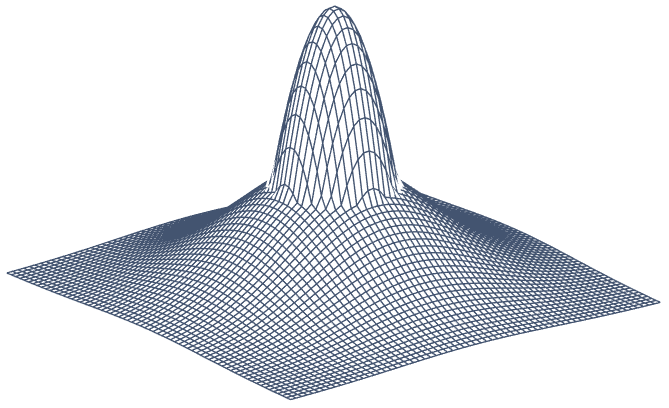
\includegraphics[scale=0.6]{Fig/BEC_manip/header.png}};
%\end{tikzpicture}

Dans la partie précédente, nous nous sommes concentrés sur la physique des atomes ultra-froids dans le désordre. En particulier, nous avons mis en évidence le fait que l'approche des atomes ultra-froids constitue une plateforme idéale pour l'étude de la propagation d'ondes dans un milieu désordonné, plateforme déjà éprouvée par l'observation de la localisation d'Anderson d'ondes de matières dans un désordre optique. 

À présent, concentrons-nous sur la description de l'un des deux éléments-clé de la propagation d'ondes dans le désordre: notre source d'ondes de matière. Le second élément, notre désordre optique, sera quant à lui présenté dans le chapitre \ref{ch:Speckle}.

Dans ce chapitre, nous nous attacherons donc à définir ce qu'est un condensat de Bose-Einstein puis nous décrirons ses principales propriétés. Dans un second temps, nous nous intéresserons aux outils dont nous disposons pour manipuler les atomes, puis nous terminerons en présentant la manière dont ces outils sont implémentés sur notre dispositif expérimental. 

\section{Condensation de Bose-Einstein}
Commençons par décrire ce qu'est un condensat de Bose-Einstein. Le phénomène de condensation a été prédit par Albert Einstein dans les années 1920 en s'appuyant sur les travaux de Satyendranath Bose traitant des statistiques quantiques pour des particules plus tard appelées \emph{bosons}. Il a cependant fallu attendre les années 1960 et le développement des premiers lasers pour voir émerger les premières techniques de manipulation d'atomes. La mise au point de telles technologies a d'ailleurs valu le prix Nobel à ses principaux architectes Claude Cohen-Tannoudji, Steven Chu et William D. Phillips en 1997. Enfin, le premier condensat de Bose-Einstein gazeux de \isotope[87]{Rb} a été obtenu par l'équipe de Eric Cornell et Carl Wieman \citep{anderson1995observation}, rapidement suivi par un condensat de \isotope[23]{Na} obtenu par Wolfgang Ketterle \citep{davis1995bose}. Ces travaux ont été récompensés par le prix Nobel de 2001.

Depuis, des condensats de Bose-Einstein ont été produits pour un grand nombre d'espèces chimique, pour des atomes comme pour des molécules. Aujourd'hui, les condensats sont couramment utilisés comme outils à des fins différentes, aussi leurs propriétés ont pu être abondamment étudiées par le passé et restent l'objet de l'investigation de plusieurs groupes dans le monde. Ainsi, nous n'en présenterons ici que les propriétés essentielles à la suite de ce manuscrit.

\subsection{Statistique de Bose-Einstein}
Le phénomène de condensation de Bose-Einstein trouve son origine dans la statistique de Bose-Einstein. Celle-ci se différencie de la statistique classique de Boltzmann dans le formalisme grand-canonique donnée par:
\begin{equation}
N_{\mathbf{n}}=g_{\mathbf{n}} \exp{\left( -(E_{\mathbf{n}}-\mu)/\kB T \right)} \text{ ,}
\end{equation}
pour un gaz de $N$ particules à l'équilibre thermique, avec $N_{\mathbf{n}}$ le nombre moyen d'atomes présents dans l'état d'énergie $E_{\mathbf{n}}$ et de dégénérescence $g_{\mathbf{n}}$, $\mu$ le potentiel chimique, $T$ la température et $\kB$ la constante de Boltzmann. L'origine de cette différence provient de l'indiscernabilité des particules: dans le cadre de la physique classique, les particules identiques sont discernables, c'est à dire qu'il est possible "d'étiqueter" les particules et de suivre leurs mouvements individuels.
Dans le cadre de la mécanique quantique, une telle approche n'est pas possible car les particules sont décrites par des fonctions d'onde, étalées dans l'espace. Lors de collisions de particules identiques, le recouvrement de leur fonction d'onde fait qu'il est impossible de déterminer les trajectoires suivies par les particules. L'indiscernabilité des particules dans le cadre de la mécanique quantique est donc essentielle.

\begin{figure}
\centering
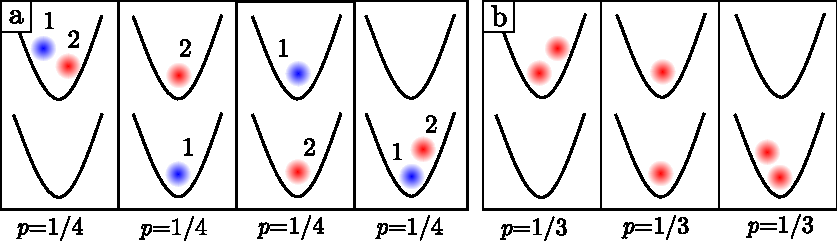
\includegraphics[width=\textwidth]{Fig/BEC_manip/stat_bose.pdf}
\caption{\textbf{a: Répartition de deux particules discernables numérotées 1 et 2 sur deux niveaux d'énergie.} Quatre configurations sont possibles. \textbf{b: Répartition de deux particules indiscernables sur deux niveaux d'énergie.} Dans le cas où ces particules peuvent se trouver dans le même état (bosons), trois configurations sont alors possibles.}
\label{fig:stat_bose}
\end{figure}

Considérons alors le cas simple de la répartition de deux particules sur deux niveaux d'énergie. Dans le cadre de la physique classique, il est possible d'attribuer un numéro à chaque particule, et il on peut placer chaque particule dans n'importe quel niveau d'énergie. Il existe alors quatre configurations que l'on supposera équiprobables, chacune de probabilité $p=1/4$ (voir figure \ref{fig:stat_bose}a). L'approche quantique, dans laquelle il n'est pas possible de discerner les particules, restreint le nombre de possibilités à trois et donc la probabilité de chacune des configurations est alors de $p=1/3$ (voir figure \ref{fig:stat_bose}b). Calculons maintenant la probabilité que deux particules soient dans le même état. En physique classique, cette probabilité est de $p=2/4=1/2$, tandis qu'en mécanique quantique, celle-ci est de $p=2/3$. On s'attend alors à ce que l'indiscernabilité des particules en mécanique quantique modifie la statistique de Boltzmann en favorisant l'agrégation de particules dans le même état \footnote{Ce raisonnement est valable pour des particules bosoniques, qui peuvent se retrouver dans le même état quantique. Pour des particules fermioniques, qui ne peuvent pas occuper le même état quantique, les statistiques en sont donc profondément changées. En guise d'illustration, la seule configuration possible de la figure \ref{fig:stat_bose}b pour des fermions est la seconde configuration.}.

\paragraph*{Condensation de Bose-Einstein}
Considérons alors le cas d'un gaz de $N$ bosons identiques dans un piège harmonique:
\begin{equation}
V(x,y,z)=\frac{1}{2}m \omega_x^2 x^2 + \frac{1}{2}m \omega_y^2 y^2 + \frac{1}{2}m \omega_z^2 z^2 \text{ ,}
\label{eq:piege_harmonique}
\end{equation}
où $m$ correspond à la masse des particules, et les $\omega_i$ correspondent aux fréquences de piégeage dans chaque direction de l'espace. Les énergies $E_{\mathbf{n}}$ sont donc celles des états liés
\begin{equation}
E_{\mathbf{n}}=\left(n_x+\frac{1}{2}\right) \hb \omega_x + \left(n_y+\frac{1}{2}\right) \hb \omega_y + \left(n_z+\frac{1}{2}\right) \hb \omega_z \quad \text{avec}\quad \mathbf{n}=\lbrace n_x,n_y,n_z\rbrace \text{ .}
\end{equation}

On peut alors montrer que le nombre moyen de particules est donné par la distribution de Bose-Einstein \footnote{Pour un gaz de $N$ fermions identiques, le nombre moyen de particules est donné par la distribution de Fermi-Dirac $ N_{\mathbf{n}}=\frac{g_{\mathbf{n}}}{\exp{\left( (E_{\mathbf{n}}-\mu)/\kB T\right)}+1}$.} \citep{diu1989elements}:
\begin{equation}
N_{\mathbf{n}}=\frac{g_{\mathbf{n}}}{\exp{\left( (E_{\mathbf{n}}-\mu)/\kB T \right)}-1} \text{ .}
\end{equation}
Une condition de validité de cette équation est que le potentiel chimique $\mu$ soit plus petit que l'énergie $E_{\mathbf{0}}$ du niveau de plus basse énergie, appelé niveau fondamental. Autrement, le nombre moyen de particules du niveau fondamental serait négatif (et cela impliquerait que la totalité du réservoir de particules vienne se déverser dans le niveau fondamental). Il est donc nécessaire que $\mu < E_{\mathbf{0}}$. Une conséquence remarquable cette condition est que la population totale des états excités est bornée par:
\begin{equation}
N_e(\mu,T)=\sum_{\mathbf{n}\neq\mathbf{0}} N_{\mathbf{n}} \leq \sum_{\mathbf{n} \neq \mathbf{0}} \frac{g_{\mathbf{n}}}{\exp{\left( (E_{\mathbf{n}}-E_{\mathbf{0}})/\kB T \right)}-1} \text{ .}
\end{equation}
Ainsi, chaque particule supplémentaire peuplera forcément l'état fondamental. On a donc ici le moyen d'accumuler un grand nombre de particules dans le même état quantique. La condensation de Bose-Einstein correspond, par définition, à cette accumulation d'un nombre macroscopique de particules dans l'état fondamental. C'est dans ce régime que les effets quantiques se manifestent, toutes ces particules partageant alors le même état quantique. Afin d'obtenir de tels effets, il est nécessaire que les fonctions d'onde des particules individuelles se recouvrent, c'est à dire que l'extension typique d'un paquet d'onde soit plus grande que la distance moyenne entre particules. Cette extension typique est donnée par la longueur d'onde thermique de de Broglie $\Delta x \sim \ldb$, qui correspond à la taille typique d'un paquet d'onde quantique dont la largeur de la distribution en impulsion est donnée par la température. Elle s'exprime \citep{diu1989elements}
\begin{equation}
\ldb=\sqrt{\frac{2\pi \hb^2}{m \kB T}} \text{ ,}
\end{equation}
avec m la masse de la particule, un atome de \isotope[87]{Rb} dans le cas de notre expérience. La distance inter-particules dans un piège est estimée à partir de la densité de particules $d \sim n^{-1/3}$. On peut alors formuler le critère phénoménologique suivant:
\begin{equation}
n \ldb^3 \gtrsim 1 \text{ .}
\label{eq:critere_condensation}
\end{equation}
La quantité $n \ldb^3$ est appelée \emph{densité dans l'espace des phases}. Tout l'enjeu des expériences d'atomes ultrafroids est d'arriver à augmenter la densité dans l'espace des phases afin de franchir le seuil donné par l'équation \ref{eq:critere_condensation}. Cette condition peut se réécrire en terme de \emph{température critique}:
\begin{equation}
T_{\mathrm{C}}\sim \frac{\hb \overline{\omega}}{\kB}N^{1/3} \text{ ,}
\label{eq:temperature_critique}
\end{equation}
où $\overline{\omega}=(\omega_x \omega_y \omega_z)^{1/3}$ est la fréquence moyenne du piège. Cette température critique est de l'ordre de quelques centaines de nanokelvin pour les expériences typiques d'atomes ultra-froids.





\subsection{Propriétés d'un condensat de Bose-Einstein}
\label{sc:propriete_BEC}
En dessous de la température critique \ref{eq:temperature_critique}, les atomes s'accumulent dans l'état fondamental du piège. Il en résulte une forte augmentation de la densité, si bien qu'on ne peut plus négliger les interactions entre particules. Dans le cas d'un gaz suffisamment dilué, ce que l'on considèrera dans la suite, les interactions entre atomes peuvent être traitées comme des collisions à basse énergie, c'est à dire des collisions uniquement dans l'onde \emph{s}. Le potentiel d'interaction est alors celui de contact, donné par $U(\mathbf{x}_1-\mathbf{x}_2)=g\delta(\mathbf{x}_1-\mathbf{x}_2)$. Le paramètre $g$, qui caractérise la force des interactions, est donné par $g=\frac{4 \pi \hb^2}{m}a_{\mathrm{s}}$, avec $a_{\mathrm{s}}$ la longueur de diffusion, et ne dépend que de ce paramètre. Ce régime dilué est atteint lorsque $na_{\mathrm{s}}^3\ll 1$\footnote{Dans ce régime, la distance inter-atomique est plus grande que la portée des interactions. Ainsi, les atomes ne voient pas le détail du potentiel d'interaction avec leur voisin, et donc il est possible d'approximer ce potentiel par un potentiel de contact.}. Pour le \isotope[87]{Rb}, cette longueur de diffusion vaut \SI{100}{\bohr}, avec \SI{}{\bohr} le rayon de Bohr. La longueur de diffusion étant positive, les interactions sont donc répulsives pour notre atome.

On peut écrire l'équation de Schrödinger pour l'état fondamental en tenant compte de ce terme d'interaction entre particules. La description en champ moyen du condensat est alors donnée par l'équation de Gross-Pitaevskii (aussi connue sous le nom d'\emph{équation de Schrödinger non-linéaire}):
\begin{equation}
\left[ -\frac{\hb^2}{2m}\Delta + V(\mathbf{x}) + g\left|\phi_0(\mathbf{x})\right|^2 \right] \phi_0(\mathbf{x}) = \mu \phi_0(\mathbf{x}) \text{ ,}
\label{eq:gross_pitaevskii}
\end{equation}
où $\phi_0(\mathbf{x})$ est la fonction d'onde macroscopique du condensat et $\mu$ est le potentiel chimique. La densité d'atomes est donnée par $n(\mathbf{x})=\left| \phi_0(\mathbf{x}) \right|^2$. Ainsi, la fonction d'onde du condensat $\phi_0(\mathbf{x})$ est normalisée pour donner le nombre de particules dans le condensat $\Nzero=\int{\diff\mathbf{x} \: \left| \phi_0(\mathbf{x}) \right|^2}$.

Le premier terme de gauche décrit l'énergie cinétique, le second le terme d'énergie potentielle provenant du piège, et le dernier décrit l'énergie d'interaction entre particules%, proportionnelle à la densité locale $n(\mathbf{x})$
. La somme de ces énergies donne le potentiel chimique $\mu$, qui correspond à l'énergie qu'il faut fournir pour rajouter une particule supplémentaire au système de $\Nzero$ particules.




\paragraph*{Régime de Thomas-Fermi}
Considérons le cas d'un condensat comportant un grand nombre de particules $\Nzero$. L'énergie cinétique totale du condensat varie avec $\Nzero$ de manière linéaire: $\mean{E_{\mathrm{k}}}\propto \Nzero$. L'énergie totale d'interaction varie quant à elle en $E_{\mathrm{int}}\propto \Nzero^2$. Pour un nombre suffisamment grand de particules, il devient possible de négliger le terme d'énergie cinétique dans l'équation de Gross-Pitaevskii stationnaire: il s'agit du régime de Thomas-Fermi.
Dans ce cas, le profil de densité s'écrit
\begin{equation}
n(\mathbf{x})=\left\{
					\begin{array}{ll}
						(\mu-V(\mathbf{x}))/g &\quad \text{lorsque} \quad \mu>V(\mathbf{x}) \text{ ,}\\
						0 &\quad \text{sinon.}
					\end{array} 
				\right.
				\label{eq:thomas_fermi}
\end{equation}
Le profil de densité est donc une parabole inversée de rayons $R_{\mathrm{TF},i}=\sqrt{\frac{2\mu}{m\omega_i^2}}$ en considérant le piège harmonique de l'équation \ref{eq:piege_harmonique}.
Ces rayons de Thomas-Fermi ont été déterminés par la condition $n(\mathbf{x})=0$. Il est intéressant de noter que le potentiel effectif vu par une particule $V_{\mathrm{eff}}(\mathbf{x})=V(\mathbf{x})+gn(\mathbf{x})$ est constant sur l'ensemble du condensat:
\begin{equation}
V_{\mathrm{eff}}(\mathbf{x})= \left\{
									\begin{array}{ll}
										\mu &\quad \text{lorsque} \quad \mu>V(\mathbf{x}) \text{ ,}\\
										V(\mathbf{x}) &\quad \text{sinon.}
									\end{array}
							\right.
\end{equation}
L'énergie d'un atome est donc constante sur l'ensemble du condensat et est donnée par le potentiel chimique. $\mu$ correspond alors à l'échelle d'énergie au-delà de laquelle le condensat est perturbé par le potentiel. Il est possible d'obtenir une expression pour le potentiel chimique \citep{pethick2008bose}: 
\begin{equation}
\mu=\frac{1}{2} \left( 15a \Nzero \hb^2 \overline{\omega}^3 \right) ^{2/5} m^{1/5} \text{ ,}
\end{equation}
qui vaut environ $\mu/h\approx\SI{40}{\hertz}$ pour notre expérience.

\begin{figure}
\centering
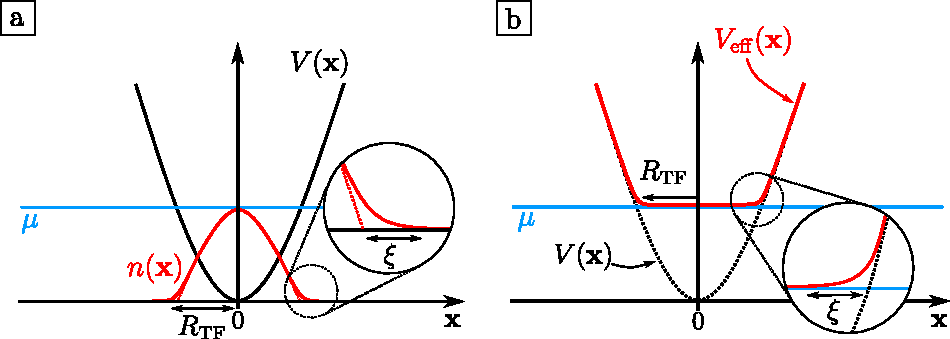
\includegraphics[width=\textwidth]{Fig/BEC_manip/thomas_fermi.pdf}
\caption{\textbf{a: Profil de densité dans le régime de Thomas-Fermi.} La densité est une parabole inversée, liée à la forme parabolique du potentiel. Sur les bords du condensat, la densité s'écarte de la parabole sur une longueur typique appelée longueur de cicatrisation \protect\footnotemark. \textbf{b: Potentiel effectif ressenti pour des particules individuelles.} Ce potentiel effectif suit la forme du potentiel externe, et l'effet des interactions à l'intérieur du condensat écrante le potentiel externe par le potentiel chimique.}
\label{fig:thomas_fermi}
\end{figure}
\footnotetext{En réalité, l'approximation de Thomas-Fermi décrit bien les zones à l'intérieur des condensats, cependant, il existe une petite région sur les bords du condensat où la densité est faible, et donc l'énergie cinétique ne peut plus être négligée devant l'énergie d'interaction. Cette échelle de longueur s'appelle la longueur de cicatrisation, et est donnée par $\xi=\sqrt{\frac{\hb^2}{n_{\mathbf{0}} mg}}$ avec $n_{\mathbf{0}}=N_{\mathbf{0}}/R_{\mathrm{TF}}^3$ la densité moyenne du condensat. $\xi$ représente donc la longueur sur laquelle le potentiel chimique n'écrante pas le potentiel externe.}








\section{Processus d'interaction lumière-matière}
Précédemment, nous avons brièvement présenté le phénomène de condensation de Bose-Einstein ainsi que les principales propriétés d'un condensat. En particulier, nous avons identifié $n \ldb^3 \gtrsim 1$ comme un critère de condensation, impliquant l'obtention de nuages denses à très basse température. Il s'agit donc de la ligne à atteindre sur notre dispositif. Dans cette partie, nous allons présenter les différents outils de manipulation d'atomes dont nous disposons, tels que des champs magnétiques, des champs lasers ou encore des radio-fréquences, afin d'obtenir la condensation d'un nuage de rubidium \isotope[87]{Rb}.

\subsection{Le rubidium \isotope[87]{Rb}}
\label{sc:Rb87}
Comme déjà mentionné plusieurs fois, l'espèce atomique utilisée sur notre expérience est le rubidium \isotope[87]{Rb}, le second isotope le plus fréquent après le rubidium \isotope[85]{Rb} (l'abondance naturelle du \isotope[87]{Rb} est de 27.8\%). Il s'agit d'un alcalin bosonique (il possède donc un seul électron de valence) avec un spin nucléaire $\mathbf{I}=3/2$. Historiquement, le \isotope[87]{Rb} est l'atome ayant été condensé en premier \citep{anderson1995observation} en raison du développement rapide des technologies laser à \SI{780}{\nano\metre}, cet atome possédant une transition optique cyclante à cette longueur d'onde dans sa raie $D$. 

La raie $D$ est en réalité composée de deux transitions: la raie $D_1$ correspondant à la transition $5^2S_{1/2}\rightarrow5^2P_{1/2}$ à \SI{795}{\nano\metre}, et la raie $D_2$ correspondant à la transition $5^2S_{1/2}\rightarrow5^2P_{3/2}$ à \SI{780}{\nano\metre}. Sauf mention contraire, nous n'utiliserons que la raie $D_2$ dans la suite de ce manuscrit, la plupart de nos fréquences optiques se trouvant autour de \SI{780}{\nano\metre}. Le choix de l'atome de rubidium est aussi dû à ses bonnes propriétés. En particulier, sa longueur de diffusion $a_{\mathrm{s}}=\SI{5.3}{\nano\metre}$ résulte en des taux de collisions relativement élevés, permettant une thermalisation rapide du nuage. 

La structure hyperfine de l'état fondamental $5^2S_{1/2}$ consiste en deux niveaux hyperfins dégénérés $\etatF{1}{}$ et $\etatF{2}{}$ séparés de $\deltahf=\SI{6.835}{\giga\hertz}$. Chacun de ces états est composé de $2F+1$ sous-états Zeeman $\etat{F,\mf}$. Une vue simplifiée de cette structure est donnée figure \ref{fig:Rb87}, et un tableau récapitulatif des principales grandeurs du \isotope[87]{Rb} peut être trouvé table \ref{tbl:Rb87}.

%\renewcommand{\arraystretch}{1.1}
\arrayrulecolor{white}
\setlength{\arrayrulewidth}{0.5mm}
\begin{table}[!ht]
\begin{center}
{\rowcolors{2}{white}{MainColor!10}
\begin{tabular}{ c|c|c }
%\hline
{\color{MainColor} \textbf{Quantité physique}} & {\color{MainColor}\textbf{Symbole}} & {\color{MainColor}\textbf{Valeur}} \\
%\hline
Masse & $m$ & \SI{1.44e-25}{\kilogram} \\
%\hline
Fréquence de transition $D_2$ & $\omega_0$ & $2\pi \times \SI{384.230}{\tera\hertz}$ \\
%\hline
Longueur d'onde dans le vide ($D_2$) & $\lambda_{\mathrm{0}}$ & \SI{780.241}{\nano\metre} \\
%\hline
Largeur naturelle de la transition $D_2$ & $\Gamma$ & $2\pi \times \SI{6.07}{\mega\hertz}$ \\
%\hline
Fréquence de transition $D_1$ & $\omega_{D_1}$ & $2\pi \times \SI{377.107}{\tera\hertz}$ \\
%\hline
Longueur d'onde dans le vide ($D_1$) & $\lambda_{D_1}$ & \SI{794.979}{\nano\metre} \\
%\hline
Largeur naturelle de la transition $D_1$ & $\Gamma_{D_1}$ & $2\pi \times \SI{5.75}{\mega\hertz}$ \\
%\hline
Séparation hyperfine & $\deltahf$ & \SI{6.834682611}{\giga\hertz} \\
%\hline
Moment cinétique nucléaire & $\mathbf{I}$ & 3/2 \\
%\hline
Facteur de Landé électronique & $g_{\mathrm{S}}$ & 2.002319 \\
%\hline
Facteur de Landé orbital & $g_{\mathrm{L}}$ & 0.999993\\
%\hline
Facteur de Landé nucléaire & $g_{\mathrm{I}}$ & \num{-0.9951414e-3} \\
%\hline
Intensité de saturation & $I_{\mathrm{sat}}$ & \SI{1.67}{\milli\watt\per\centi\metre^2} \\
%\hline
Longueur de diffusion & $a_{\mathrm{s}}$ & \SI{5.3}{\nano\metre} \\
%\hline
\end{tabular}}
\end{center}
\caption{Tableau récapitulatif des grandeurs physiques du rubidium \isotope[87]{Rb} que nous utiliserons dans la suite. Ces valeurs sont tirées de \citep{steck2001rubidium}.}
\label{tbl:Rb87}
\end{table}

\begin{figure}
\centering
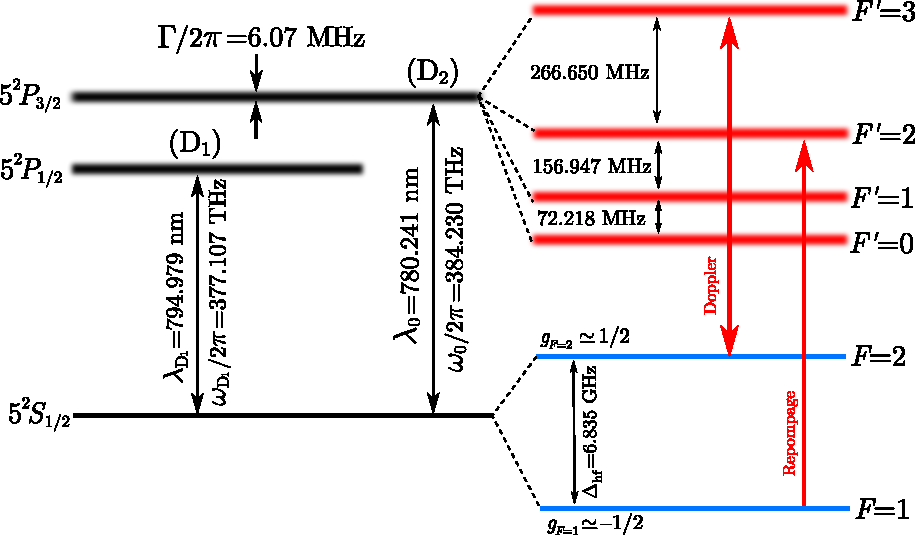
\includegraphics[width=0.8\textwidth]{Fig/BEC_manip/Rb87.pdf}
\caption{\textbf{Structure de la raie $D$ du rubidium \isotope[87]{Rb}.} Celle-ci est composée de deux transitions, la $D_1$ à \SI{795}{\nano\metre}, et la transition $D_2$ à \SI{780}{\nano\metre} que nous utilisons sur l'expérience. L'état fondamental $5^2S_{1/2}$ est dégénéré en deux sous-niveaux hyperfins séparés d'une énergie $h \deltahf$ avec $\deltahf=\SI{6.835}{\giga\hertz}$.}
\label{fig:Rb87}
\end{figure}

\subsection{Potentiel magnétique}
Commençons par décrire l'interaction d'un atome de rubidium avec un champ magnétique statique. Ces champs magnétiques sont couramment utilisés dans les expériences d'atomes ultra-froids pour réaliser des pièges conservatifs à l'aide champs inhomogènes (après un refroidissement laser par exemple). En particulier, l'expérience de Stern \& Gerlach montre que la force appliquée aux atomes par un gradient de champ magnétique dépend de l'état interne de l'atome. Explicitons cela.

Le moment cinétique total $\hat{\mathbf{F}}$ est donné par la somme des moments cinétiques des composants de l'atome:
\begin{equation}
\hat{\mathbf{F}}=\hat{\mathbf{I}}+\hat{\mathbf{L}}+\hat{\mathbf{S}} \text{ ,}
\end{equation}
avec $\hat{\mathbf{I}}$ le spin total nucléaire, $\hat{\mathbf{L}}$ le moment cinétique orbital et $\hat{\mathbf{S}}$ le moment cinétique de spin électronique. On a alors un moment magnétique total $\hat{\boldsymbol\mu}=\mub (g_{\mathrm{I}} \hat{\mathbf{I}} + g_{\mathrm{L}} \hat{\mathbf{L}} + g_{\mathrm{S}} \hat{\mathbf{S}})$ où les $g_{\mathrm{I},\mathrm{L},\mathrm{S}}$ sont les facteurs de Landé et $\mub$ est le magnéton de Bohr\footnote{L'interaction avec le spin du noyau donne une correction très faible car $g_{\mathrm{I}}\propto 1/m_{\mathrm{P}}$ avec $m_{\mathrm{p}}$ la masse du proton, et $g_{\mathrm{L,S}} \propto 1/m_{\mathrm{e}}$ avec $m_{\mathrm{e}}$ la masse de l'électron. Ainsi, $g_{\mathrm{I}} \ll g_{\mathrm{L,S}}$ (voir table \ref{tbl:Rb87}), on pourra donc en général négliger l'effet du spin nucléaire lors de l'application d'un champ magnétique extérieur.}. L'énergie d'interaction de ce moment magnétique avec un champ magnétique $\mathbf{B}$ est donnée par $\hat{V}=-\hat{\boldsymbol\mu}.\mathbf{B}$. On obtient les énergies propres par la formule de Breit-Rabi, dont l'application aux états hyperfins $\etatF{1}{}$ et $\etatF{2}{}$ fournit:
\begin{equation}
\begin{aligned}
E_{F=2} &= + \frac{h \deltahf}{2} \sqrt{1+ m_F \beta +\beta^2} \\
E_{F=1} &= - \frac{h \deltahf}{2} \sqrt{1+ m_F \beta +\beta^2} \text{ ,}
\end{aligned}
\label{eq:Breit-Rabi}
\end{equation}
avec $\beta \simeq 2 \mub \left| B \right| /h \deltahf$. À faible champ magnétique $\left| B \right| \ll h \deltahf / \mub$ (régime où $\beta \ll 1$), on retrouve l'effet Zeeman linéaire avec
\begin{equation}
U_{\mathrm{mag}} (\mathbf{x}) = \mf g_{\mathrm{F}} \mub \left| B(\mathbf{x}) \right| \text{ ,}
\end{equation}
et $g_{\mathrm{F}=2}= 1/2$ et $g_{\mathrm{F}=1} =-1/2$. L'utilisation d'un champ magnétique non homogène génère donc un potentiel dépendant de la position, tel que dans l'expérience de Stern \& Gerlach. L'utilisation de tels champs inhomogènes est très répandue dans le domaine des atomes ultra-froids, en particulier pour la génération de pièges magnétiques, l'accélération de particules, mais aussi pour réaliser une lévitation magnétique comme c'est le cas sur notre expérience. 







\subsection{Forces lumineuses}
\label{sc:forces_lumineuses}
On se concentre à présent sur l'interaction entre un atome et un champ laser incident. Ce champ laser comporte un grand nombre de photons émis par seconde (typiquement \num{e12} photons par seconde pour une puissance de \SI{1}{\micro\watt}), on peut donc décrire ce champ laser par une onde classique 
\begin{equation}
\mathbf{E}(\mathbf{x},t)= \mathrm{Re} \left( E(\mathbf{x}) e^{-i \omega t - i\phi (\mathbf{x})}  \boldsymbol\epsilon \right) \text{ ,}
\end{equation}
dont l'effet sur un atome est donné par le hamiltonien $H_{\mathrm{AL}}=-\mathbf{D}.\mathbf{E}(\mathbf{x},t)$. 
Dans la cadre de la théorie de la réponse linéaire, on introduit la polarisabilité atomique $\alpha(\omega)$ et on montre alors que la force moyenne exercée sur un atome est la somme de deux termes:
\begin{equation}
\mathbf{F}=\frac{1}{2} \mathrm{Re}(\alpha(\omega)) E(\mathbf{x}) \nabla E(\mathbf{x})+\frac{1}{2}\mathrm{Im}(\alpha(\omega)) E^2(\mathbf{x}) \nabla \phi(\mathbf{x}) \text{ .}
\label{eq:forces_lumineuses}
\end{equation}
Un calcul pleinement quantique est nécessaire pour déterminer la polarisabilité $\alpha(\omega)$, et il est possible de montrer que pour un système à deux niveaux, on a \citep{grimm2000optical}:
\begin{equation}
\alpha(\omega)=6 \pi \epsilon_0 c^3 \frac{\Gamma / \omega_0^2}{\omega_0^2 -\omega^2 -i(\omega^3/\omega_0^2)\Gamma} \text{ ,}
\end{equation}
où $\omega_0$ est la fréquence de résonance et $\Gamma$ est la largeur de la transition.

\paragraph*{Potentiel dipolaire}
Le premier terme de l'équation \ref{eq:forces_lumineuses} est proportionnel à la partie réelle de la polarisabilité atomique. Ce terme décrit donc comment un moment dipolaire électrique induit interagit avec le gradient d'intensité lumineuse. Cette force est conservative et dérive d'un potentiel qui est proportionnel à l'intensité lumineuse: on parle de \emph{potentiel dipolaire}. Dans le cas d'un faisceau très désaccordé, ce potentiel s'écrit:
\begin{equation}
U_{\mathrm{dip}}(\mathbf{x})=\frac{3\pi c^2 I(\mathbf{x})}{2 \omega_0^3} \left( \frac{\Gamma}{\omega - \omega_0} - \frac{\Gamma}{\omega + \omega_0} \right) \text{ ,}
\label{eq:potentiel_dipolaire}
\end{equation}
avec $I(\mathbf{x})$ l'intensité lumineuse à la position $\mathbf{x}$. Cette expression est valable très loin de résonance: cela signifie que le laser ne voit pas le détail de la raie $D$ du \isotope[87]{Rb}, c'est à dire que le désaccord $\omega-\omega_0$ doit être très grand devant la structure fine séparant les transitions $D_1$ et $D_2$, et l'onde laser ne voit qu'un système à deux niveaux $\lbrace 5 {}^2S, 5 {}^2P \rbrace$.

Un tel potentiel présente de nombreux avantages pour les expériences d'atomes ultrafroids. Suivant le signe de la quantité $\delta = \omega-\omega_0$, ce potentiel peut être soit attractif ($\delta<0$, on parlera alors de potentiel désaccordé vers le \emph{rouge}), soit répulsif ($\delta>0$, potentiel désaccordé vers le \emph{bleu}). Les atomes seront alors attirés par les maximas d'intensité lumineuse (pour un faisceau désaccordé vers le rouge) ou bien vers les zones d'ombre (pour les faisceaux désaccordés vers le bleu). Un faisceau gaussien focalisé et désaccordé vers le rouge permet ainsi de piéger les atomes en son foyer: la forme gaussienne du faisceau attire les atomes vers le centre du faisceau. 

De plus dans cette limite des grands désaccords, ce potentiel est indépendant de l'état interne. Contrairement à un piège magnétique, un piège dipolaire n'est pas sélectif en état de spin et donc offre de nombreuses possibilités grâce à la disponibilité de degrés de liberté internes. Nous tirerons profit de cet avantage de différentes manières dans la suite. 

Cependant, l'utilisation de tels désaccords (plusieurs centaines de nanomètres) nécessite de très fortes intensités lumineuses afin d'obtenir des potentiels suffisamment importants. Ainsi, il est courant que les expériences d'atomes ultrafroids utilisent des lasers possédant une puissance de plusieurs Watts\footnote{À titre de comparaison, il ne suffit que de quelques \SI{}{\milli\watt} pour endommager l'œil humain.} focalisés sur de petites tailles, typiquement de l'ordre de $10-\SI{100}{\micro\metre}$. 

\begin{comment}
Il se pose alors la question de la dissipation, liée à l'émission spontanée. Le taux d'émission spontanée peut être estimé par:
\begin{equation}
\Gamma_{\mathrm{sp}}(\mathbf{x})=\frac{3 \pi c^2 I(\mathbf{r})}{2\hb \omega_0^3} \left( \frac{\omega}{\omega_0}\right)^3 \left( \frac{\Gamma}{\omega-\omega_0}-\frac{\Gamma}{\omega+\omega_0} \right)^2
\end{equation}
et dans le cas dans d'un faisceau très désaccordé on peut souvent négliger ce taux et la dissipation qui lui est associée.
\end{comment}
Insistons sur le fait que l'expression \ref{eq:potentiel_dipolaire} a été obtenue dans le contexte d'un système à deux niveaux, et que cette approximation n'est valable que dans la limite des grands désaccords pour un atome de \isotope[87]{Rb}. Un laser faiblement désaccordé ($\sim \SI{1}{\nano\metre}$) peut ainsi sonder la structure fine, voire la structure hyperfine de l'atome. Cela permet des approches originales telles que la réalisation d'un potentiel dépendant de l'état interne, que nous présenterons section \ref{sc:state_dependent_disorder}. %En revanche, le rapprochement des transitions atomiques rend les atomes susceptibles de subir des processus de diffusions inélastiques de photons via l'émission spontanée, décrits plus bas.


%%%%%%%%%%%%%%%%%%%%%%%%%%%%%%%%%%%%
\begin{comment}
L'utilisation de désaccords plus modérés, typiquement de quelques nano-mètres, permet de fortement diminuer la puissance optique utilisée. En revanche, un tel rapprochement de la transition atomique implique qu'on ne peut plus négliger l'effet de la structure fine de la raie $D$. On peut alors considérer l'atome comme un système à non plus deux mais trois niveaux en négligeant la structure hyperfine de l'atome pour des désaccords gardés suffisamment grands $\omega-\omega_0 \gg \Delta_{\mathrm{hf}}$ et $\omega-\omega_{D_1} \gg \Delta_{\mathrm{hf}}$ (les séparations hyperfines des états excités sont plus petites que la séparation hyperfine des états fondamentaux).

Pour de tels désaccords et pour un faisceau polarisé linéairement, le potentiel dipolaire est alors donné par
\begin{equation}
U_{\mathrm{dip}}(\mathbf{r})=\frac{\pi c^2 I(\mathbf{r})}{2\omega_0^3} \left( \frac{\Gamma_{D_1}}{\omega-\omega_{D_1}} - \frac{\Gamma_{D_1}}{\omega+\omega_{D_1}} + \frac{2\Gamma}{\omega-\omega_0}-\frac{2\Gamma}{\omega+\omega_0}\right)
\end{equation}
Une conséquence de la structure fine est l'existence d'une zone entre les deux transitions où le potentiel est tantôt répulsif, tantôt attractif suivant que la fréquence du laser se rapproche de la fréquence de transition $D_1$ (répulsif) ou de la transition $D_2$ (attractif). Il existe donc une région dans laquelle il est possible de passer d'un potentiel désaccordé vers le bleu à un potentiel décalé vers le rouge sans croiser une transition atomique, comme illustré figure \ref{fig:v_dip_magique}. De plus, entre ces domaines de potentiel attractif et répulsif, il existe une longueur d'onde dite \emph{magique} pour laquelle le potentiel s'annule (les contributions des transitions $D_1$ et $D_2$ se compensent). Cette longueur d'onde est d'environ \SI{790}{\nano\metre} et peut être un véritable outil des expériences d'atomes ultrafroids, pour la réalisation d'un potentiel dépendant de l'état interne par exemple.

\begin{figure}
\centering
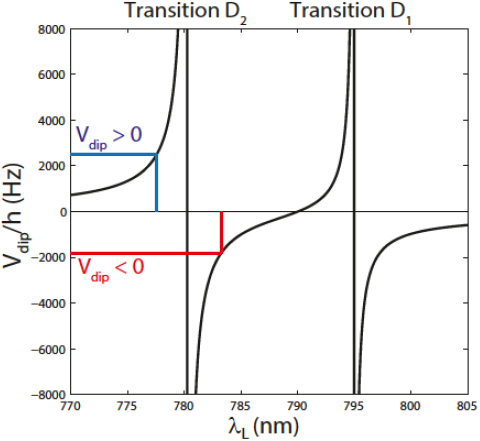
\includegraphics[scale=0.6]{Fig/BEC_manip/V_dip.png}
\caption{\textbf{Potentiel dipolaire en fonction de la longueur d'onde du laser.} La présence des deux transitions est remarquable par les deux divergences. Elles sont séparées par une zone de potentiel tantôt attractif, plus répulsif. Entre ces deux régimes se trouve une longueur d'onde \emph{magique} à environ \SI{790}{\nano\metre} pour laquelle le potentiel s'annule, quelque soit la puissance du laser.}
\label{fig:v_dip_magique}
\end{figure}

Naturellement, le rapprochement des transitions atomiques entraîne une augmentation du taux d'émission spontanée. Pour les désaccords considérés, il s'exprime
\begin{equation}
\Gamma_{\mathrm{sp}}=\frac{\pi c^2 I(\mathrm{r})}{2 \hb \omega_0^3} \left[ \left(\frac{\omega}{\omega_{D_1}} \right)^3 \left( \frac{\Gamma_{D_1}}{\omega-\omega_{D_1}} - \frac{\Gamma_{D_1}}{\omega+\omega_{D_1}} \right)^2 + 2\left( \frac{\omega}{\omega_0} \right)^3 \left( \frac{\Gamma}{\omega-\omega_0}-\frac{\Gamma}{\omega+\omega_0} \right)^2 \right]
\end{equation}
et l'ordre de grandeur du temps de vie associé est de l'ordre de quelques secondes.


Notons enfin qu'il est possible de se rapprocher encore plus de résonance et de devenir sensible à la structure hyperfine de la transition $D_2$ (dans ces conditions on peut négliger la contribution de la raie $D_1$). En revanche, le taux d'émission spontanée croît fortement et devient très contraignant.

\end{comment}
%%%%%%%%%%%%%%%%%%%%%%%%%%%%%%%%%%%


\paragraph*{Force de pression de radiation}
Le second terme s'appelle \emph{force de pression de radiation}. Il provient de la partie imaginaire de la polarisabilité atomique, qui caractérise l'absorption de photons par l'atome. Il s'agit donc d'une force inélastique qui résulte d'un grand nombre de cycles d'absorption de photons du faisceau laser et d'émission spontanée dans des directions aléatoires de l'espace \footnote{Pour réaliser de tels cycles, il est nécessaire d'avoir une transition cyclante, c'est à dire de disposer d'un état excité dont la désexcitation renvoie forcément sur l'état d'origine.}. L'impulsion totale cédée par émission spontanée s'annule donc, et en moyenne le transfert d'impulsion ne provient que de l'absorption de photons du faisceau laser. Ceci est illustré par le terme de droite de l'équation \ref{eq:forces_lumineuses}, faisant apparaître le gradient de la phase du laser $\boldsymbol{\nabla} \phi (\mathbf{x})=\mathbf{k}$. 

On montre que cette force s'exprime \citep{cohen2012processus}:
\begin{equation}
\mathbf{F}_{\mathrm{PR}}=\hb \mathbf{k} \Gamma_{\mathrm{sp}} \text{ ,}
\end{equation}
avec $\Gamma_{\mathrm{sp}}$ le taux d'émission spontanée en présence du champ laser, et $\mathbf{k}$ le vecteur d'onde associé à l'onde laser. L'interprétation est directe: en moyenne, l'atome acquiert une impulsion $\hb \mathbf{k}$ à un taux $\Gamma_{\mathrm{sp}}$. Ce taux vaut:
\begin{equation}
\Gamma_{\mathrm{sp}}=\frac{\Gamma}{2} \frac{s}{1+s} \quad \text{avec} \quad s=\frac{I/I_{\mathrm{sat}}}{1+4\delta^2/\Gamma^2} \text{ ,}
\end{equation}
où l'intensité de saturation $I_{\mathrm{sat}}=\frac{\pi h c \Gamma}{3\lambda_0^3}=\SI{1.67}{\milli\watt\per\centi\metre^2}$ est une constante de l'atome de \isotope[87]{Rb}. La grandeur $s$ s'appelle le paramètre de saturation. Celui-ci dépend de l'intensité lumineuse incidente (et donc du nombre de photons incidents) ainsi que du désaccord du laser par rapport à la résonance atomique\footnote{L'expression \ref{eq:potentiel_dipolaire} n'est valable que dans un régime de faible saturation. L'utilisation de grands désaccords autorise l'utilisation de grosses puissances optiques tout en gardant $s\ll 1$. Dans ce régime, on peut estimer le taux d'émission spontanée par $\Gamma_{\mathrm{sp}}(\mathbf{x})=\frac{3 \pi c^2 I(\mathbf{x})}{2\hb \omega_0^3} \left( \frac{\omega}{\omega_0}\right)^3 \left( \frac{\Gamma}{\omega-\omega_0}-\frac{\Gamma}{\omega+\omega_0} \right)^2$.} $\delta = \omega-\omega_0$.  Le paramètre de saturation est maximal en $\delta=0$, c'est à dire lorsque le laser est à résonance. Dans le cas d'un laser très saturant $s \gg 1$, la force de pression de radiation s'écrit
\begin{equation}
\mathbf{F}_{\mathrm{PR}}=\frac{\hb \mathbf{k} \Gamma}{2} \text{ ,}
\end{equation}
où le facteur 2 indique que à forte saturation, un atome autant de chance d'être dans l'état excité que dans l'état fondamental. Enfin, mentionnons que pour un atome se déplaçant à une vitesse $\mathbf{v}$ dans le référentiel du laboratoire, le désaccord devient $\delta=\omega-\omega_0-\mathbf{k}.\mathbf{v}$ par effet Doppler. Nous reviendrons sur ce point lorsque nous décrirons les mécanismes du refroidissement laser.





\subsection{Couplage radio-fréquence} 
Les outils de manipulation des atomes présentés précédemment offrent la possibilité de créer des potentiels conservatifs (comme le potentiel dipolaire ou le potentiel magnétique) ou encore des forces dissipatives à l'aide la force de pression de radiation. De manière générale, certains de ces outils dépendent de l'état interne des atomes\footnote{Le potentiel magnétique dépend bien évidemment de l'état interne, tandis que ce n'est pas de le cas du potentiel dipolaire dans la limite des grands désaccords.}, une dernière possibilité de manipulation des atomes consiste donc à contrôler leur état électronique.% Un bon contrôle de ce degré de liberté permet donc d'augmenter l'efficacité des processus qui en dépendent (le chargement d'un piège magnétique par exemple), ainsi que de proposer des solutions technologiques originales. 

Comme présenté section \ref{sc:Rb87}, la séparation entre les états fondamentaux $\etatF{1}{}$ et $\etatF{2}{}$ correspond à une fréquence $\deltahf$ de l'ordre du \SI{}{\giga\hertz}, donc à une fréquence qui se trouve accessible électroniquement. Il apparaît alors possible de contrôler de l'état interne des atomes à l'aide d'un rayonnement radio-fréquence. L'effet de ce couplage sur les atomes peut être décrit par un système à deux niveaux dont le hamiltonien\footnote{Le terme de couplage \ref{eq:hamiltonien_rabi} est obtenu en appliquant l'approximation de l'onde tournante, c'est à dire que l'on néglige les termes en $\omega +2\pi\Delta_{\mathrm{hf}}$ devant les termes en $\omega - 2\pi\Delta_{\mathrm{hf}}$ car on estime qu'ils évoluent rapidement, et donc qu'ils s'apparentent à leur valeur moyenne qui est nulle.} est donné dans la base $\etatF{1}{}, \etatF{2}{}$ par 
\begin{equation}
\hat{H}(t)=\frac{\hb}{2} \begin{pmatrix}
-2\pi\Delta_{\mathrm{hf}} & \Omega e^{i \omega t} \\
\Omega e^{-i\omega t} & 2\pi\Delta_{\mathrm{hf}}
\end{pmatrix} \text{ ,}
\label{eq:hamiltonien_rabi}
\end{equation}
avec $\omega$ la pulsation de l'onde radio-fréquence, et $\Omega$ la pulsation de Rabi qui caractérise l'amplitude rayonnée sur les atomes.  En se plaçant dans le référentiel tournant, le hamiltonien du système devient
\begin{equation}
\hat{H}=\frac{\hb}{2} \begin{pmatrix}
\delta & \Omega \\
\Omega & -\delta
\end{pmatrix} \text{ ,}
\end{equation}
avec $\delta=\omega- 2\pi\deltahf$. En supposant que le système est dans l'état $\etatF{1}{}$ à $t=0$, la probabilité d'avoir l'atome dans l'état $\etatF{2}{}$ est donnée par la formule de Rabi \citep{basdevant2002mecanique}:
\begin{equation}
\mathcal{P}_{\etatF{2}{}}(t)= \frac{\Omega^2}{\Omega^2+\delta^2} \sin^2{\left(\sqrt{\Omega^2+\delta^2} \frac{t}{2} \right) } \text{ .}
\label{eq:rabi_formule}
\end{equation}
Cette formule met en évidence un caractère résonant des transitions radio-fréquences:
\begin{itemize}
\item[\textendash] Dans le cas d'un grand désaccord $\delta \gg \Omega$, la probabilité de transition est très faible à n'importe quel instant.
\item[\textendash] À résonance $\delta=0$, la probabilité de transition peut atteindre 1, même pour un couplage très faible ($\Omega$ petit).
\end{itemize}
La formule de Rabi \ref{eq:rabi_formule} est tracée figure \ref{fig:rabi} en représentations temporelle et spectrale, et permet d'en illustrer les caractéristiques. Notamment, la figure \ref{fig:rabi}.a témoigne des oscillations de la probabilité de transition avec une amplitude dépendant du désaccord $\delta$. 
En particulier, l'enveloppe lorentzienne de la probabilité maximale de transition en fonction de $\delta$ est représentée en pointillés noirs figure \ref{fig:rabi}.b. On montre ainsi que la probabilité maximale de transition ne peut être atteinte qu'à résonance ($\delta=0$), et que celle-ci décroît en augmentant le désaccord.

\begin{figure}
\centering
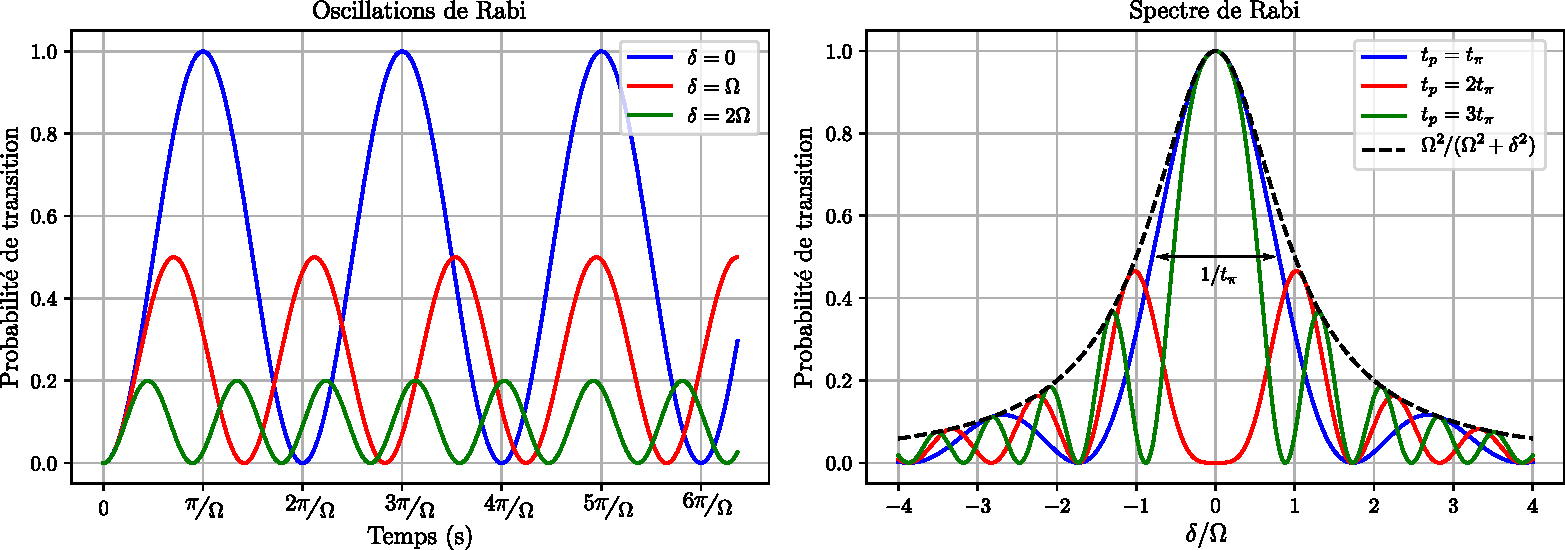
\includegraphics[width=\textwidth]{Fig/BEC_manip/rabi.pdf}
\caption{\textbf{a: Oscillations de Rabi tracées pour différents désaccords.} Les populations oscillent à la pulsation $\sqrt{\Omega^2+\delta^2}$ avec une amplitude qui dépend du désaccord. L'amplitude est maximale et atteint 1 lorsque l'onde radio-fréquence est à résonance, et la population maximale transférée décroît avec l'augmentation du désaccord. \textbf{b: Spectres de Rabi pour différentes durées d'application $\boldsymbol{t_p}$.} Le transfert de population est le plus efficace à résonance ($\delta=0$), et l'utilisation d'un désaccord entraîne une diminution de l'efficacité de transfert. Les populations maximales transférées sont décrites par l'enveloppe lorentzienne de l'équation \ref{eq:rabi_formule}.}
\label{fig:rabi}
\end{figure}






\section{Description d'un cycle expérimental}
Dans la partie précédente, nous nous sommes familiarisés avec quelques outils couramment utilisés sur les expériences d'atomes ultra-froids pour piéger et manipuler les atomes. Dans cette nouvelle partie, nous nous pencherons sur l'implémentation de ces outils sur notre expérience afin d'obtenir un condensat de Bose-Einstein de \isotope[87]{Rb}. La présentation qui en est donnée ici se verra minimale, nous nous contenterons d'illustrer brièvement les différentes étapes de refroidissement qui mènent à la condensation. De nombreux détails pourront être trouvés dans les thèses des doctorants qui ont contribué à faire de cette expérience ce qu'elle est aujourd'hui: \citep{fauquembergue2004realisation}\citep{riou2006etude}\citep{bernard2010transport}\citep{jendrzejewski2012quantum}\citep{muller2015coherent}\citep{denechaud2018vers}\citep{mukhtar2019state}.

\subsection{Présentation générale du dispositif}
Comme toutes les expériences d'atomes ultra-froids, la manipulation des atomes se déroule sous ultra-vide afin de s'affranchir des conditions extérieures. En particulier, on évite ainsi les collisions avec des particules extérieures à température ambiante, ce qui chaufferait notre gaz et détruirait la cohérence d'un nuage condensé. Une vue d'ensemble de l'enceinte à vide est donnée figure \ref{fig:manip} qui montre aussi les pompes utilisées en continu pour maintenir le vide. Notre dispositif est composé d'un four chauffé à \SI{120}{\degreeCelsius} qui éjecte les atomes de rubidium, il s'agit de notre source d'atomes. Un doigt froid refroidi à \SI{-30}{\degreeCelsius} sert de diaphragme et permet de filtrer le jet d'atomes tout en adsorbant les atomes qui sont bloqués afin de pas polluer le vide. Un obturateur mécanique permet de couper le jet lorsqu'on ne souhaite pas accumuler des atomes en cours de cycle. Les atomes sont décélérés dans le ralentisseur Zeeman et capturés dans la première cellule où ils subissent les premières étapes de refroidissement. Ils sont ensuite transportés dans la seconde cellule où ils sont refroidis jusqu'à la condensation. C'est dans cette seconde cellule que se déroulent les expériences de science, on l'appelle alors \emph{Chambre de science}.

\begin{figure}
\centering
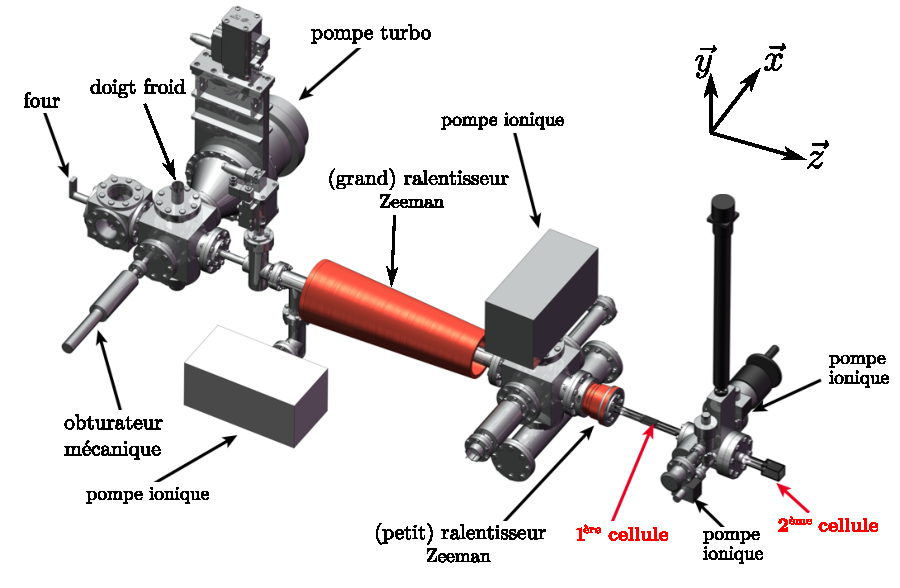
\includegraphics[width=\textwidth]{Fig/BEC_manip/manip.pdf}
\caption{\textbf{Vue d'ensemble du corps de l'expérience.} Les atomes se trouvent dans un montage sous ultra-vide, composé de deux chambres dans lesquelles les atomes sont manipulés.}
\label{fig:manip}
\end{figure}

\subsection{Première chambre}
C'est dans la première chambre que se déroulent les premières étapes de refroidissement du gaz de rubidium. Celles-ci sont dans un premier temps basées sur le refroidissement laser, puis dans un second temps sur un piégeage magnétique et l'évaporation forcée à l'aide d'un couteau radio-fréquence.

\paragraph*{Refroidissement laser}
Le principe du refroidissement laser repose sur la force de pression de radiation, présentée section \ref{sc:forces_lumineuses}. Plus particulièrement, le refroidissement laser consiste à dissiper de l'énergie cinétique à l'aide de cycles d'absorption et d'émission spontanée de photons. 

Considérons le cas d'un atome se déplaçant à vitesse $\mathbf{v}$ dans le référentiel du laboratoire soumis à une onde laser contrapropageante de pulsation $\omega$. Le désaccord du laser par rapport à la transition atomique s'exprime $\delta=\omega-\omega_0- \mathbf{k}. \mathbf{v}$, où le décalage Doppler $\mathbf{k}.\mathbf{v}<0$. Dans le référentiel de l'atome, la condition de résonance $\delta=0$ s'écrit $\omega_0=\omega-\mathbf{k}.\mathbf{v}$. L'atome va alors absorber un photon laser d'énergie $\hb \omega$ et en émettre un d'énergie supérieure $\hb \omega_0$ par émission spontanée. Il y a donc eu un transfert d'énergie entre l'énergie cinétique et le désaccord. La répétition de tels cycles permet ainsi de transférer beaucoup d'énergie cinétique de l'atome vers le désaccord entre photons absorbés et photons rayonnés.

La possibilité de répéter ces cycles d'absorption de photons et d'émission spontanée repose sur l'existence d'une transition cyclante entre les états hyperfins $\etatF{2}{}$ et $\etat{F'=3}$. La désexcitation de $\etat{F'=3}$ renvoie forcément l'atome dans l'état $\etatF{2}{}$ car les règles de sélection imposent $F'-F= \lbrace 0, \pm 1 \rbrace$.
En revanche, on peut accidentellement envoyer des atomes dans l'état excité $\etat{F'=2}$ car la séparation avec l'état ciblé $\etat{F'=3}$ n'est que de \SI{266}{\mega\hertz}. Statistiquement, un atome visite cet état tous les 50 cycles environ, et sa désexcitation peut faire tomber les atomes dans l'état $\etatF{1}{}$. Cet état étant un état noir, pour conserver les atomes, on doit alors utiliser un second laser appelé \emph{repompeur} qui permet de recycler les atomes perdus vers la transition cyclante\footnote{À titre d'illustration, le temps de vie du piège magnéto-optique a été mesuré à une dizaine de secondes. Sans le faisceau repompeur, les atomes tombent dans l'état noir $\etatF{1}{}$ en quelques micro-secondes seulement.}. Il est accordé sur la transition $\etatF{1}{} \rightarrow \etat{F'=2}$.

Notre dispositif laser se compose alors d'un laser principal de refroidissement accordé sur la transition $\etatF{2}{} \rightarrow \etat{F'=3}$. Il est secondé d'un second laser \emph{repompeur} accordé sur la transition $\etatF{1}{} \rightarrow \etat{F'=2}$. Enfin un dernier laser sert de référence de fréquence pour les deux précédents en étant asservi par absorption saturée. Une représentation schématique de l'ensemble de ces lasers et de leur amplification peut être trouvée figure \ref{fig:table_optique}.

\begin{figure}
\centering
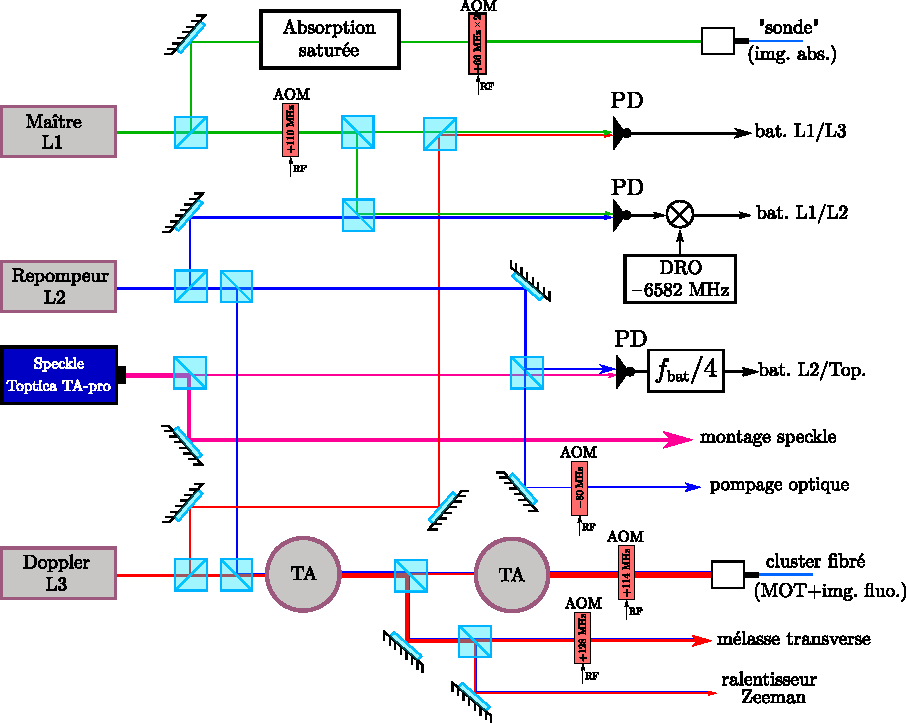
\includegraphics[width=0.8\textwidth]{Fig/BEC_manip/table_optique2.pdf}
\caption{\textbf{Représentation schématique de notre montage laser.} Le laser maître \emph{L1} sert de référence de fréquence en étant asservi par absorption saturée. Le laser de refroidissement Doppler \emph{L3} est asservi par battements avec \emph{L1}. Le laser repompeur \emph{L2} est lui aussi asservi par battements avec \emph{L2} grâce à l'utilisation d'électronique rapide. Notons enfin que les faisceaux de \emph{L2} et \emph{L3} sont mélangés avant amplification (TA). Les faisceaux arrivant sur les atomes comporteront alors les fréquences provenant de ces deux lasers. Un obturateur mécanique (non représenté) permet de couper le faisceau de \emph{L2} allant vers les amplificateurs.}
\label{fig:table_optique}
\end{figure}

\paragraph*{Le ralentisseur Zeeman}
La première étape consiste à ralentir suffisamment le jet d'atomes pour pouvoir les capturer dans un premier piège. Un laser désaccordé vers le rouge par rapport à la transition cyclante $\etatF{2}{} \rightarrow\etat{F'=3}$ permet de réaliser une décélération des atomes à l'aide de cycles d'absorption et d'émission spontanée de photons. Cependant, le ralentissement des atomes désaccorde le faisceau laser de la résonance atomique par effet Doppler. Pour palier à ce problème, on applique un champ magnétique pour satisfaire localement la condition de résonance par effet Zeeman\footnote{D'autres solutions furent envisagées lors des premiers développement des expériences d'atomes froids. Parmi celles-ci, mentionnons les faisceaux lasers \emph{chirpés} \citep{ertmer1985laser} et les lasers spectralement larges \citep{zhu1991continuous}.}. Ce champ est appliqué à l'aide d'une bobine comportant un nombre de tours par unité de longueur variable, représentée figure \ref{fig:manip} entre le four et la première chambre.
Ainsi, on est capable de réduire la vitesse des atomes de \SI{100}{\metre\per\second} à environ \SI{20}{\metre\per\second} sur une distance de seulement \SI{1}{\metre}.

\paragraph*{Le piège magnéto-optique}
Une fois les atomes suffisamment ralentis, ils sont capturés dans le piège magnéto-optique (abrégé en \emph{MOT} pour l'anglais \textit{Magneto-Optical Trap}). Celui-ci est composé de trois paires de faisceaux contra-propageants désaccordés vers le rouge d'environ $\delta=\SI{-16}{\mega\hertz}$, de polarisations opposées $\sigma^+$ et $\sigma^-$. Chacun de ces faisceaux possède une puissance d'environ \SI{12}{\milli\watt}.
De plus, deux bobines en configuration anti-Helmholtz permettent de générer un champ quadrupolaire, donc un gradient magnétique dans les trois directions de l'espace, afin de créer une force de rappel.
On charge environ \num{2e9} atomes en moins d'une seconde grâce à la mélasse transverse qui permet de collimater le jet d'atomes et donc d'améliorer le flux. 
Une fois le chargement saturé, on coupe le champ magnétique pendant quelques millisecondes afin de réduite fortement la température: c'est l'étape de mélasse optique qui permet de descendre la température à environ \SI{50}{\micro\kelvin}. 

\begin{figure}
\centering
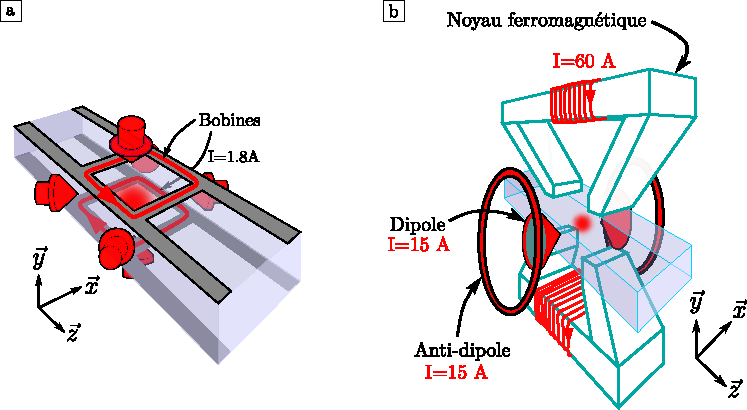
\includegraphics[width=\textwidth]{Fig/BEC_manip/MOT_magtrap.pdf}
\caption{\textbf{a: Éléments du piège magnéto-optique.} Il est réalisé à l'aide de trois paires de faisceaux contra-propageants et de deux bobines formant un champ quadrupolaire. Ces bobines sont faites à partir de circuits imprimés posés sur la cellule. \textbf{b: Géométrie du piège magnétique.} Un champ quadrupolaire intense est créé selon les directions $\vec{y}$ et $\vec{z}$ par un électroaimant. Un champ de biais est généré par deux paires de bobines suivant la direction $\vec{x}$. Ce champ possède une courbure longitudinale et est responsable du confinement suivant cette direction. }
\label{fig:MOT_magtrap}
\end{figure}

\paragraph*{Piège magnétique et évaporation radio-fréquence}
À l'issue de l'étape de mélasse, les atomes sont chargés dans un piège magnétique qui va permettre de se rapprocher considérablement du seuil de condensation. Afin d'augmenter le nombre d'atomes piégeables magnétiquement, il est nécessaire de manipuler l'état interne des atomes. On procède ainsi à une étape de dépompage en éteignant le faisceau de repompage et en accordant le faisceau de refroidissement sur la transition $\etatF{2}{} \rightarrow\etat{F'=2}$: en moins d'une milliseconde, les atomes se trouvent dans l'état $\etatF{1}{}$, dont seul le sous-état Zeeman $\etatF{1}{-1}$ peut être piégé\footnote{Il est le seul des trois sous-états Zeeman de $\etatF{1}{}$ à avoir le produit $g_{\mathrm{F}} \mf > 0$, c'est à dire qu'il s'agit d'un état \emph{Low Field Seeker}, qui est attiré par les zones de faible champ magnétique. En effet, c'est à l'aide d'un minimum de champ magnétique que l'on réalise ce piège, le théorème de Wing interdisant les maximas de champ magnétique. }\footnote{Des huit sous-états Zeeman fondamentaux, il s'agit de celui ayant la plus grande probabilité d'occupation tout en étant piégeable, justifiant son choix. }. Afin de maximiser la population de ce sous-état, on allume un faisceau de pompage optique accordé sur la transition $\etatF{1}{} \rightarrow \etat{F'=1}$ et polarisé $\sigma^-$ pendant \SI{40}{\micro\second}. En parallèle, on allume le champ du \emph{dipôle} afin de définir un axe de quantification.

Le piège magnétique que l'on utilise est un piège de type \emph{Ioffe-Pritchard}. Il est composé essentiellement de deux éléments:
\begin{itemize}
\item[\textendash] Un champ de biais orienté dans la direction $\vec{x}$, généré par une paire de bobines (\emph{dipôle}) de configuration légèrement plus éloignée que celle de Helmholtz: on a ainsi une courbure positive dans la direction longitudinale au centre des bobines. Une seconde paire de bobines (\emph{anti-dipôle}) permet d'abaisser le champ constant au centre du piège sans changer significativement sa courbure. Cet abaissement du biais magnétique se traduit par une compression du nuage \citep{fauquembergue2004realisation}.
\item[\textendash] Un champ quadrupolaire dans le plan $(\vec{y},\vec{z})$ généré par un électroaimant ferromagnétique épais (\emph{quadrupôle}) comportant deux entrefers et deux bobines excitatrices dans deux sens opposés. L'épaisseur importante du matériau magnétique minimise l'effet de l'électroaimant dans la direction $\vec{x}$.
\end{itemize}
Le confinement dans la direction $\vec{x}$ est donc réalisée par le champ de \emph{dipôle}\footnote{Notons que la présence du champ de dipôle permet aussi de s'affranchir des pertes par transition Majorana, le champ ne s'annulant à aucun endroit de l'espace.}, tandis que le confinement dans les directions $\vec{y}$ et $\vec{z}$ est fait par le \emph{quadrupôle}. 
On obtient ainsi un nuage piégé magnétiquement comportant environ \num{1e9} atomes tous dans le même sous-état zeeman à une température de $\sim \SI{300}{\micro\kelvin}$.

Une fois le nuage thermalisé, on procède à une étape de refroidissement évaporatif grâce à la méthode de \emph{couteau radio-fréquence}. Une étude détaillée du refroidissement évaporatif est proposée section \ref{sc:evap_optique}, mais on peut en résumer le principe, illustré figure \ref{fig:evapRF}, de la manière suivante:
\begin{itemize}
\item[\textendash]On tronque le piège de telle sorte que quelques atomes très énergétiques (la queue de la distribution de vitesses de Maxwell-Boltzmann) puissent s'en échapper, chaque atome emportant une énergie supérieure à l'énergie moyenne par atome.
\item[\textendash]Les collisions entre les particules étant restées dans le piège permettent au système de thermaliser. Ce nouvel état d'équilibre thermique est caractérisé par une température plus basse.
\end{itemize}

La troncature du piège se fait à l'aide d'une onde radio-fréquence rayonnée par les bobines MOT. Celle-ci induit une transition de l'état piégé $\etatF{1}{-1}$ à l'état non piégé $\etatF{1}{0}$ lorsque la condition de résonance $\hb \omega_{\mathrm{RF}} = \mf g_{\mathrm{F}} \mub B(\mathbf{x})$ est vérifiée. En abaissant progressivement la fréquence rayonnée pendant une dizaine de secondes, on obtient finalement un nuage d'environ \num{70e6} atomes à une température de \SI{10}{\micro\kelvin}.

\begin{figure}
\centering
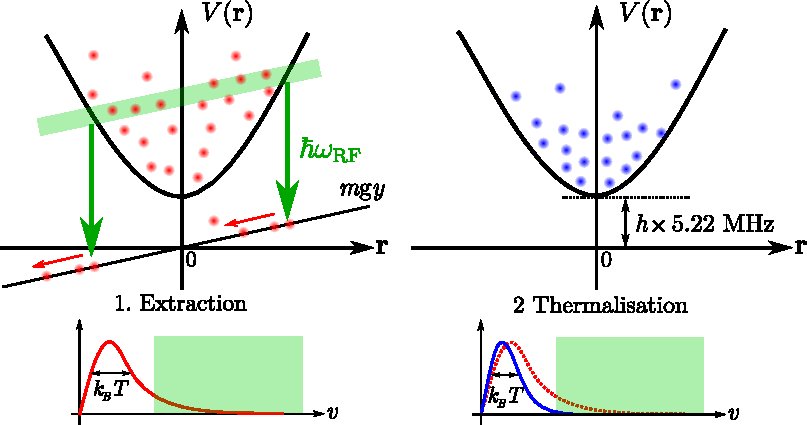
\includegraphics[width=0.9\textwidth]{Fig/BEC_manip/evapRF.pdf}
\caption{\textbf{Principe de l'évaporation radio-fréquence.} L'application d'une radio-fréquence permet de tronquer le piège magnétique, et d'éliminer les atomes les plus énergétiques. L'énergie moyenne par particule étant plus basse, la température s'en retrouve abaissée après thermalisation.}
\label{fig:evapRF}
\end{figure}


\subsection{Chambre de science}
\label{sc:chambre_science}
Après ces premières étapes de refroidissement, les atomes sont transportés dans une seconde cellule où l'on procède à une évaporation tout-optique pour franchir le seuil de condensation. La raison d'être de cette seconde cellule est de profiter d'un maximum d'accès optiques tout en s'affranchissant de l'environnement magnétique de la première chambre, en particulier celui du ferromagnétique.

Nous nous contenterons ici de présenter les grandes lignes des éléments de cette seconde chambre, de nombreux détails pourront être trouvés dans la thèse d'Alain Bernard \citep{bernard2010transport}, dans la thèse de Fred Jendrzejewski \citep{jendrzejewski2012quantum} et de Kilian Muller \citep{muller2015coherent}. Certains de ces éléments ont fait l'objet de modifications au cours de ma thèse, aussi une étude plus approfondie en sera présentée dans le chapitre \ref{ch:new_exp}.

\paragraph*{Transport dans une pince optique et piège dipolaire croisé}
Après évaporation radio-fréquence, on transfert le nuage dans une pince optique. Il s'agit d'un piège dipolaire créé par focalisation sur les atomes d'un faisceau laser de longueur d'onde $\lambda=\SI{1070}{\nano\metre}$ et de puissance estimée d'environ \SI{1.5}{\watt}. Dans le plan focal, ce faisceau a une taille $\mathrm{w}_{\mathrm{0}}=\SI{28}{\micro\metre}$ et la distance de Rayleigh vaut donc $z_{\mathrm{R}}= \pi \mathrm{w}_{\mathrm{0}}^2 / \lambda=\SI{2.3}{\milli\metre}$. On obtient ainsi \num{10e6} atomes à une température de \SI{10}{\micro\kelvin} aux alentours du foyer de la pince\footnote{Ce faible taux de transfert entre le piège magnétique et la pince provient du mauvais recouvrement spatial entre ces deux pièges. La pince est très allongée suivant la direction $\vec{z}$, tandis que le piège magnétique est étendu suivant la direction $\vec{x}$. Cette géométrie est un héritage des débuts de cette expérience, originellement utilisée pour étudier le laser à atomes.}.

Le transport dans la seconde chambre se fait à l'aide d'une platine de translation montée sur coussin d'air \emph{Aerotech ABL80040}. Les optiques de focalisation de la pince se trouvant sur cette platine, on déplace ainsi les atomes de \SI{40}{\centi\metre} en moins de \SI{2}{\second}, comme illustré figure \ref{fig:piege_optique}. On estime l'efficacité de transfert à 75\%.%, mesurée en effectuant un aller-retour pour retourner dans la première chambre.

\begin{figure}
\centering
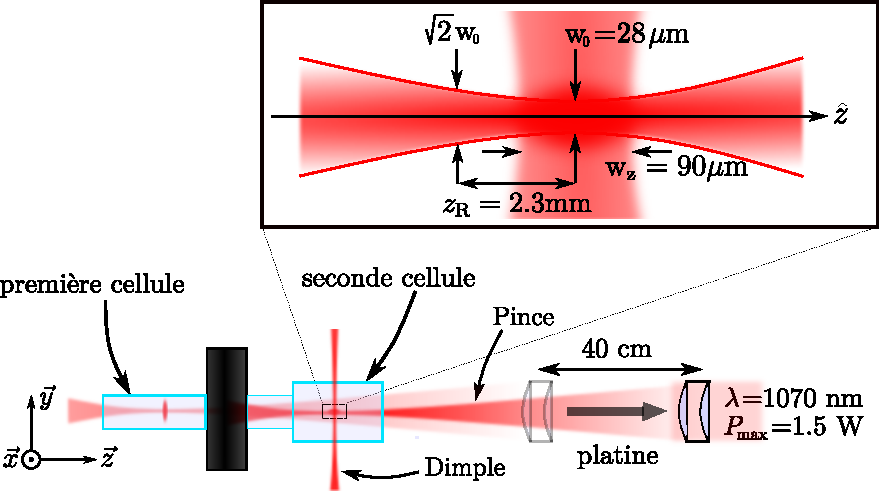
\includegraphics[width=0.9\textwidth]{Fig/BEC_manip/piege_optique2.pdf}
\caption{\textbf{Illustration du transport et du piège optique.} Les atomes sont capturés autour du foyer de la pince dans la première chambre, et le point de focalisation est déplacé de \SI{40}{\centi\metre} à l'aide d'une platine de translation. Une fois le transport terminé, on allume un second faisceau de piégeage vertical (\emph{dimple}).}
\label{fig:piege_optique}
\end{figure}

Une fois les atomes arrivés dans la seconde chambre, un second faisceau de piégeage dipolaire de longueur d'onde \SI{1070}{\nano\metre} et de puissance \SI{7}{\watt} est allumé afin de comprimer le nuage suivant la direction $\vec{z}$ qui correspond à la direction longitudinale de la pince. Ce faisceau \emph{Dimple} est de forme elliptique, de tailles $\SI{180}{\micro\metre} \times \SI{90}{\micro\metre}$ dans les directions $\vec{x}$ et $\vec{z}$ respectivement. Étant donnée sa grande longueur de Rayleigh (de l'ordre du centimètre), on suppose que le piégeage vertical induit est négligeable devant toutes les autres sources de piégeage. Ainsi, dans le piège dipolaire croisé, le confinement suivant les directions $\vec{x}$ et $\vec{y}$ est fait par la pince, tandis que le confinement suivant la direction $\vec{z}$ est fait par le faisceau vertical\footnote{La forme allongée du dimple dans la direction $\vec{x}$ fait que le piégeage dans cette direction est très faible comparé à celui de la pince. De plus, cela rend le piège optique tolérant face à un léger défaut d'alignement.}, comme illustré figure \ref{fig:piege_optique}. À ce stade, on estime disposer de \num{3e6} atomes à une température de \SI{10}{\micro\kelvin}.

Enfin, une dernière étape d'évaporation est requise pour franchir le seuil de condensation. Succinctement, celle-ci consiste à diminuer la puissance des lasers afin de diminuer la profondeur des potentiels de piégeage de telle sorte que les atomes les plus énergétiques puissent s'échapper. La description et l'optimisation de cette étape feront l'objet de la partie \ref{sc:evap_optique}.



\paragraph*{Lévitation magnétique}
Une contrainte forte de l'étude la localisation d'Anderson réside dans les grands temps de propagation dans le désordre nécessaires pour pouvoir qualifier un état de localisé. Dans l'expérience visant à observer la localisation d'Anderson à trois dimensions, l'évolution du nuage dans le désordre a pu être suivie pendant plusieurs secondes \citep{jendrzejewski2012three}, ce qui n'est possible qu'en compensant la gravité. En conséquence, notre expérience dispose d'une lévitation magnétique. Celle-ci a été mise en place durant la thèse d'Alain Bernard et de nombreux détails concernant ce système et ses performances se trouvent dans son manuscrit. Cependant, la lévitation magnétique a fait l'objet d'une attention particulière durant ma thèse, aussi une étude approfondie en sera donnée dans la partie \ref{sc:levitation}. Donnons en tout de même quelques caractéristiques.

Le principe de la lévitation magnétique est de compenser la force de pesanteur à l'aide d'un gradient magnétique. Pour l'état $\etatF{1}{-1}$ qui est \emph{Low Field Seeker}, il s'agit d'un gradient de \SI{30}{\gauss\per\centi\metre}. Cependant, la conservation du flux magnétique $\boldsymbol{\nabla} . \mathbf{B}=0$ induit des gradients dans les autres directions. Ceci impose une valeur minimale aux fréquences de piégeage par le biais du théorème de Wing \citep{sackett2006limits}:
\begin{equation}
\sum_{i=x,y,z} \omega_i^2 \geq \left| \frac{mg^2}{2 \mf g_{\mathrm{f}} \mub \Bzero}\right| \text{ ,}
\label{eq:theoreme_wing}
\end{equation} 
avec $g$ l'accélération de la pesanteur et $B_0$ la norme du champ magnétique à la position des atomes. Une stratégie de réduction de ces fréquences de piégeage (les $\omega_i$ sont positifs pour l'état $\etatF{1}{-1}$) consiste à augmenter fortement le champ $\Bzero$. On utilise alors des bobines supplémentaires pour générer un tel champ, qui peut monter jusqu'à \SI{2000}{\gauss}, réduisant les fréquences de piégeage à environ $\omega_i /2 \pi \sim \SI{0.2}{\hertz}$. Une version simpliste du design de notre lévitation est donnée figure \ref{fig:levitation_simple}.

Une autre stratégie couramment utilisée par l'équipe est de se placer dans l'état $\etatF{2}{-2}$ qui est \textit{High Field Seeker}, il sera donc expulsé de la lévitation par les courbures résiduelles. Il s'agit pour nous d'un avantage puisque cela favorise le processus d'évaporation, de plus on ne pourra pas attribuer à la lévitation un éventuel arrêt de l'expansion du nuage dans l'étude de la localisation d'Anderson. Pour atteindre cet état, on applique une transition radio-fréquence dans le piège optique croisé avant évaporation.

\begin{figure}
\centering
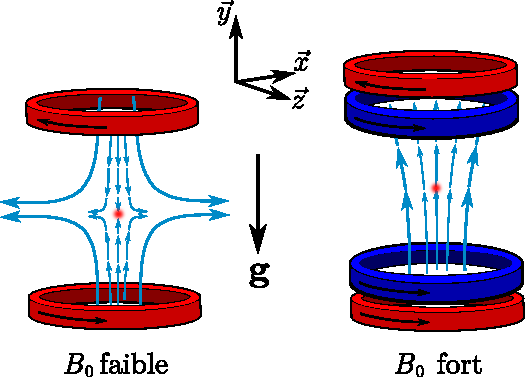
\includegraphics[scale=1]{Fig/BEC_manip/levitation_simple.pdf}
\caption{\textbf{Design simplifié de la lévitation magnétique}. Un gradient magnétique est appliqué aux atomes grâce à une paire de bobines parcourues par des courants opposés (en rouge). La conservation du flux magnétique entraîne des gradients dans les autres directions de l'espace. L'application d'un fort champ de biais créé par d'autres bobines (en bleu) permet de minimiser l'impact de ces gradients et de diminuer les fréquences de piégeage (ou d'anti-piégeage) associées.}
\label{fig:levitation_simple}
\end{figure}

Pour finir, citons un dernier avantage offert par la lévitation magnétique: la compensation de la gravité permet de ne pas "pencher" le potentiel de notre piège optique. Nous avons donc la possibilité de pousser l'évaporation optique jusque dans un domaine où la gravité aurait normalement dû tirer les atomes en dehors du piège, permettant ainsi d'évaporer beaucoup plus loin et d'atteindre des pièges optiques très peu profonds et très décomprimés.



\paragraph*{Refroidir encore plus}
L'assimilation d'un condensat de Bose-Einstein à une onde de matière monochromatique $\etat{\mathbf{k}=0}$ nécessite de pouvoir négliger l'énergie des atomes devant l'amplitude du désordre (voir section \ref{sc:etat_art_transition}), et implique donc d'obtenir des nuages extrêmement froids. Bien que la lévitation magnétique nous permette d'obtenir des nuages particulièrement décomprimés, le refroidissement peut être poussé encore plus loin. 

Une première technique consiste en une décompression du nuage à l'aide de l'ouverture adiabatique du piège. Cette décompression se traduit par une diminution des fréquences de piégeage, que l'on obtient en changeant la taille des faisceaux de piégeage. En pratique, il nous suffit de reculer le plan de focalisation de la pince de \SI{4.5}{\milli\metre} en \SI{1}{\second} à l'aide de la platine de translation comme illustré figure \ref{fig:adia_opening_and_delta_kick}a. La température obtenue est alors donnée par le théorème d'équipartition de l'énergie:
\begin{equation}
T'=\frac{\omega_{\mathrm{r}}'}{\omega_{\mathrm{r}}}T < T \text{ ,}
\end{equation}
avec $\omega_{\mathrm{r}}$ la fréquence de piégeage de la pince dans la direction radiale. L'abaissement de la température est donc obtenu par diminution de la densité du nuage, c'est à dire par dilution. Cette étape se déroule en même temps que l'évaporation optique.

À la fin du cycle d'évaporation et d'ouverture adiabatique, il reste environ \num{2e5} atomes dont environ 50\% forment un condensat de Bose-Einstein. Le potentiel chimique de la partie condensée est estimée à $\mu/h=\SI{40}{\hertz}$, et la température de la fraction thermique est d'environ \SI{5}{\nano\kelvin}. 

\begin{figure}
\centering
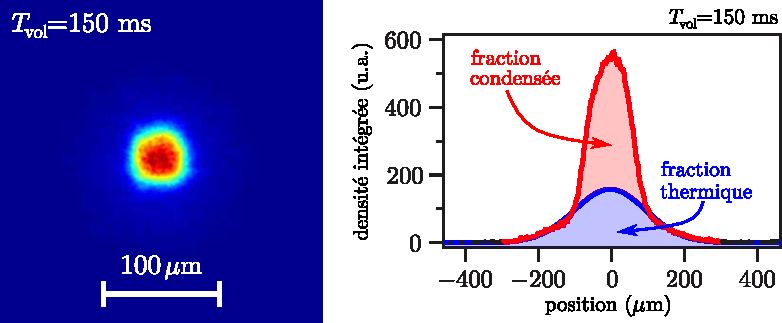
\includegraphics[width=0.9\textwidth]{Fig/BEC_manip/BEC_double_struct.pdf}
\caption{\textbf{Image expérimentale d'un condensat de Bose-Einstein}. Cette image correspond à celle d'un condensat après expansion pendant un temps de vol de \SI{150}{\milli\second}. L'image de droite correspond au profil de la densité intégrée suivant une direction, et montre la double structure témoignant d'une partie condensée. La partie condensée a un profil parabolique (en rouge), tandis que la partie thermique est de forme gaussienne (en bleu).}
\label{fig:BEC_double_struct}
\end{figure}

Après l'extinction du piège, l'énergie d'interaction du nuage est convertie en énergie cinétique, le nuage s'étend alors librement dans le champ de lévitation. L'évolution de la taille du nuage donne alors accès à la distribution de vitesse, en particulier à sa dispersion $\Delta k \simeq \SI{0.5}{\per\micro\metre}$. 

Une seconde technique, basée sur le principe de focalisation atomique par un potentiel harmonique, permet de réduire davantage cette dispersion. Cette technique dite de \emph{refroidissement par delta-kick} consiste à transférer l'énergie d'interaction en énergie cinétique en éteignant le piège, puis à figer le mouvement des atomes en appliquant un potentiel harmonique pendant un bref instant. L'énergie cinétique est alors transformée en énergie potentielle. Une illustration de ce procédé est donnée figure \ref{fig:adia_opening_and_delta_kick}b.

Une approche classique permet de justifier cela. En supposant que l'expansion des atomes est balistique, la position des atomes après un grand temps d'expansion $t_{\mathrm{exp}}$ est donnée par leur vitesse initiale\footnote{L'utilisation de temps d'expansion $t_{\mathrm{exp}}$ tels que le déplacement des atomes soit très grand devant la taille initiale du nuage permet de s'affranchir de cette dernière, voir annexe \ref{ch:anex_mesure_temp}.}:
\begin{equation}
\mathbf{x}(t_{\mathrm{exp}})=\mathbf{v} t_{\mathrm{exp}} \text{ .}
\end{equation}
Appliquons un kick de potentiel harmonique pendant un temps $\Delta t$. La vitesse des atomes à la fin de ce kick est donnée par
\begin{equation}
\dot{\mathbf{x}}(\Delta t) = -\mathbf{x} \omega \sin{(\omega \Delta t)}+ \mathbf{v} \cos{(\omega \Delta t)} \text{ ,}
\end{equation}
avec $\omega$ la fréquence du piège.
On peut trouver $\Delta t$ tel que $\dot{\mathbf{x}}_i=0$:
\begin{equation}
\Delta t= \frac{1}{\omega} \arctan{\left(\frac{1}{t_{\mathrm{exp}} \omega} \right)} \text{ .}
\end{equation}
On remarque que $\Delta t$ ne dépend pas de la vitesse initiale des atomes: on peut donc geler l'ensemble du nuage en appliquant un potentiel harmonique pendant la bonne durée de kick\footnote{Une approche équivalente consiste à dire que la force de rappel est proportionnelle à la distance parcourue par les atomes, qui est proportionnelle à la vitesse initiale. L'instant où les vitesses s'annulent ne dépend donc pas de la vitesse initiale des atomes.}. 
La mise en œuvre expérimentale de cette technique est détaillée dans le manuscrit de thèse de Kilian Muller \citep{muller2015coherent} et témoigne de résultats impressionnants: la dispersion en vitesse s'est abaissée à $\Delta k \simeq \SI{0.15}{\per\micro\metre}$. La température effective associée est alors de $T\sim \SI{150}{\pico\kelvin}$, et en tenant compte de la taille du nuage de l'ordre de $\Delta x \sim \SI{30}{\micro\metre}$, on s'approche à un ordre de grandeur de la limite de Heisenberg $\Delta x \hb \Delta k \simeq 10 \hb /2$.

\begin{figure}
\centering
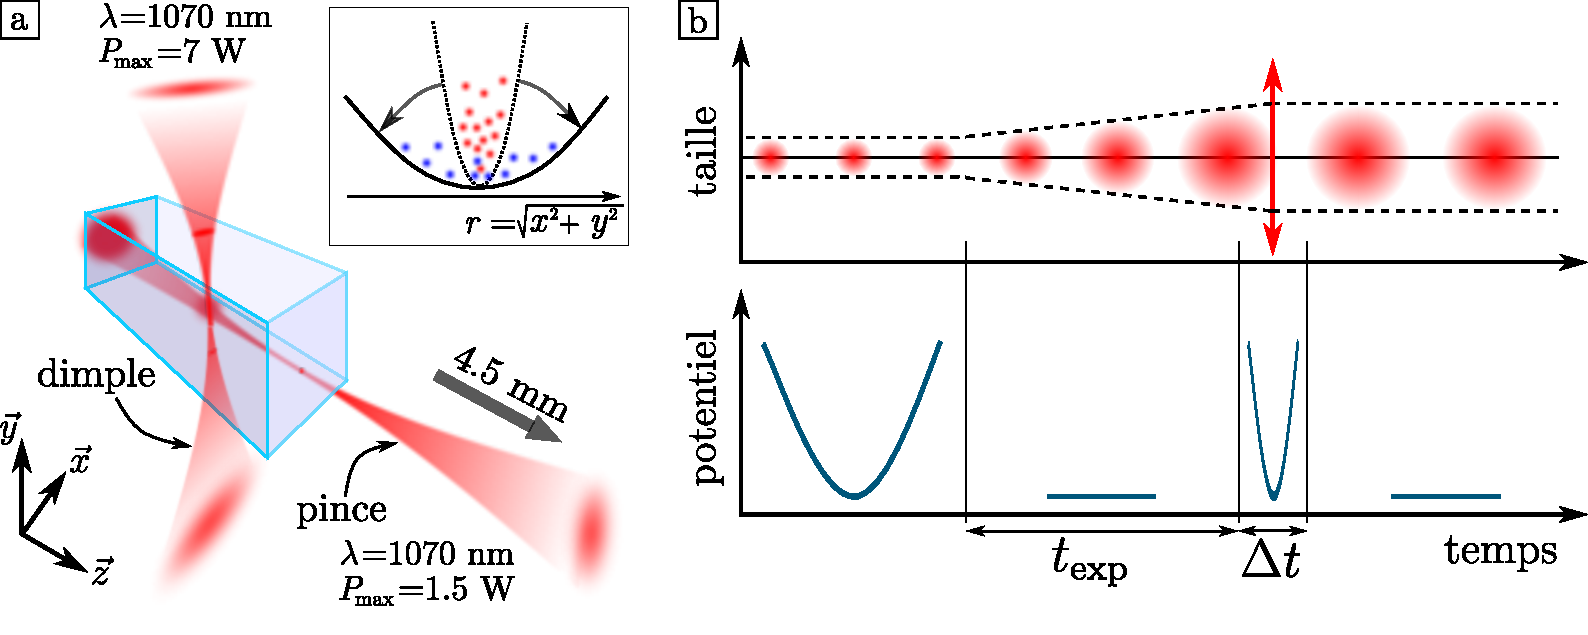
\includegraphics[width=\textwidth]{Fig/BEC_manip/adia_opening_and_delta_kick2.pdf}
\caption{\textbf{a: Principe de l'ouverture adiabatique.} Le déplacement du point de focalisation de la pince permet d'augmenter la taille du faisceau au niveau des atomes. La fréquence de piégeage en est alors diminuée, et on abaisse alors la température par dilution. \textbf{b: Illustration du refroidissement par \emph{delta-kick}.} L'extinction du piège entraîne l'étalement du nuage, et le transfert de l'énergie d'interaction en énergie cinétique. On peut ensuite \textit{focaliser} les atomes à l'aide d'un \textit{kick} de potentiel, en transformant l'énergie cinétique en énergie potentielle, supprimée à l'extinction du piège.}
\label{fig:adia_opening_and_delta_kick}
\end{figure}















\subsection{Imagerie}
\label{sc:imagerie}
Nos cycles expérimentaux se concluent par une étape de mesure, nous permettant d'obtenir des informations à propos de notre gaz d'atomes. Une grande partie de ces informations peut être extraite d'une image du nuage après extinction du piège (voir annexe \ref{ch:anex_mesure_temp}), image que l'on obtient à l'aide d'une caméra et l'utilisation de lasers à résonance avec les atomes \footnote{L'utilisation de lasers à résonance conduit inévitablement à la destruction du nuage sur notre expérience. Il est donc nécessaire de répéter l'ensemble du cycle expérimental pour obtenir une seconde image des atomes.}. %L'utilisation d'un retard (appelé \emph{temps de vol} et abrégé en \emph{TOF} pour l'anglais \textit{Time Of Flight}) entre l'extinction du piège et la prise de l'image est extrêmement courant fournit de précieux renseignements.

\paragraph*{Implémentation expérimentale de l'imagerie}
L'expérience est équipée de trois caméras \textit{EMCCD C9102} de \textit{Hamamatsu}, chacune comportant une matrice de $1000 \times 1000$ pixels de taille $\SI{8}{\micro\metre} \times \SI{8}{\micro\metre}$. Ces trois caméras sont contrôlées via l'outil d'acquisition d'images du logiciel \emph{MATLAB}, qui permet aussi de récupérer et traiter les images obtenues. L'acquisition des images est déclenchée de manière externe par un second ordinateur pilotant l'ensemble de l'expérience.

Une première caméra acquiert des images des atomes dans la première chambre selon l'axe horizontal $\vec{x}$ avec un grandissement de 1, la zone imageable est donc de $\SI{8}{\milli\metre} \times \SI{8}{\milli\metre}$. Il est possible d'utiliser cette caméra pour de l'imagerie par absorption (représentée figure \ref{fig:img_mot}) ainsi que pour de l'imagerie par fluorescence grâce à un montage 4$f$. Néanmoins, l'observation selon une direction induit forcément une intégration de la densité suivant cette direction: on ne peut mesurer qu'une densité intégrée
\begin{equation}
n_{\mathrm{2D}}(y,z) =\int{\mathrm{d}x \: n(x,y,z)} \text{ ,}
\end{equation}
avec $n$ la densité à trois dimensions.

Les deux dernières caméras sont disposées autour de la chambre de science selon l'axe horizontal $\vec{x}$ et l'axe vertical $\vec{y}$. Toutes deux voient le nuage au travers d'un système optique de grandissement 3\footnote{Ce grandissement a été mesuré on observant la chute libre du nuage en l'absence de la lévitation.}, conduisant à une résolution de \SI{2.7}{\micro\metre} pour une zone imageable de $\SI{2.7}{\milli\metre} \times \SI{2.7}{\milli\metre}$. Seule de l'imagerie par fluorescence est utilisable dans cette chambre, en revanche il est possible d'utiliser ces deux caméras simultanément pour obtenir les densités intégrés suivant deux directions $n_{\mathrm{2D}}(y,z)$ et $n_{\mathrm{2D}}(x,y)$ pour le même nuage.

\paragraph*{Imagerie par absorption}
Le principe de l'imagerie par absorption repose sur la loi de Beer-Lambert
\begin{equation}
I((y,z)= I_0(y,z) \times \exp{(-\sigma n_{\mathrm{2D}}(y,z))} \text{ ,}
\end{equation}
avec $\sigma$ la section efficace d'absorption des atomes. En effet, lorsque qu'un faisceau laser traverse un milieu, son absorption dépend directement de la densité du milieu en particules absorbantes (la densité atomique dans notre cas). Pour sonder cette densité atomique, on envoie donc un faisceau laser à résonance directement sur les atomes et la caméra comme illustré figure \ref{fig:img_mot}. 

\begin{figure}
\centering
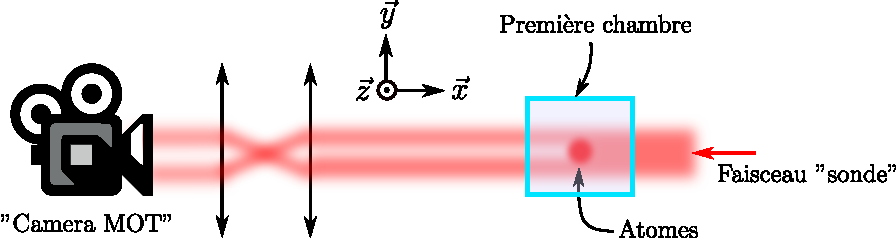
\includegraphics[width=\textwidth]{Fig/BEC_manip/img_mot.pdf}
\caption{\textbf{Imagerie par absorption.} Un faisceau collimaté est envoyé sur les atomes, qui absorbent une partie des photons qui traversent le nuage. Le signal détecté à la caméra correspond à "l'ombre" des atomes, et la comparaison avec une image du faisceau incident sans atomes permet de remonter à la densité atomique intégrée selon la direction longitudinale.}
\label{fig:img_mot}
\end{figure}

Dans un régime de très basse saturation $s \ll 1$, on peut montrer que la section efficace d'absorption des atomes $\sigma$ est indépendante de l'intensité incidente $I_0(y,z)$ et $\sigma\approx\SI{2.9e-9}{\centi\metre^2}$ \citep{steck2001rubidium}. En pratique, on s'assure d'être dans le régime de basse saturation en gardant la puissance du faisceau \emph{sonde} inférieure à \SI{100}{\micro\watt}. Le faisceau \emph{sonde} correspond à une impulsion lumineuse d'une durée de \SI{50}{\micro\second} réalisée par un laser à résonance avec la transition $\etatF{2}{} \rightarrow \etat{F'=3}$\footnote{Puisque le faisceau sonde est à résonance avec la transition $\etatF{2}{} \rightarrow \etat{F'=3}$, celui-ci ne permet de détecter que les atomes se trouvant dans l'état $\etatF{2}{}$. Afin de mesurer aussi les atomes qui sont dans l'état $\etatF{1}{}$, on procède à un transfert de population vers l'état $\etatF{2}{}$ à l'aide d'une impulsion du faisceau repompeur accordé sur la transition $\etatF{1}{} \rightarrow \etat{F'=2}$ pendant une durée de \SI{40}{\micro\second}. Ce transfert est réalisé \SI{100}{\micro\second} avant le déclenchement de la caméra. }.



L'application de la loi de Beer-Lambert permet de déterminer la densité atomique intégrée suivant l'axe d'imagerie:
\begin{equation}
n_{\mathrm{2D}}(y,z)= \frac{1}{\sigma} \mathrm{ln}\left( \frac{I_0(y,z)}{I(y,z)} \right) \text{ .}
\end{equation}
L'opération de reconstruction du profil de densité atomique nécessite donc deux images: une première image des atomes absorbant une partie du faisceau \emph{sonde}, puis une seconde image du même faisceau sans les atomes pour en déterminer le profil d'intensité $I_0(y,z)$. En pratique, une troisième image est utilisée afin de soustraire le bruit de fond. % en raison de la faible puissance optique.% De plus, une bonne reconstruction du profil nécessite des contraintes supplémentaires. En effet, nous nous fixons de travailler dans un régime où la sonde ne sature pas la caméra (cela fixe une borne supérieure pour l'intensité du faisceau), et où l'absorption de photons n'est pas totale dans les régions les plus denses.



\paragraph*{Imagerie par fluorescence}
Le principe de l'imagerie par fluorescence consiste à éclairer les atomes avec de la lumière à résonance, puis à détecter la lumière que les atomes diffusent à l'aide d'un système optique de grande ouverture numérique, comme illustré figure \ref{fig:img_science}. Un avantage de cette technique par rapport à l'imagerie par absorption est sa capacité à détecter de très faibles nombres d'atomes, rendu possible grâce à l'amplification des caméras. Un deuxième avantage réside dans la simplicité de sa mise en œuvre: dans la première chambre, l'imagerie par fluorescence est réalisée à l'aide des faisceaux MOT. L'imagerie de la seconde chambre est quant à elle réalisée à l'aide de deux autres faisceaux dédiés. Les faisceaux d'imagerie consistent en une impulsion lumineuse d'une durée de \SI{50}{\micro\second}, fortement saturante $s\gg 1$ et accordée sur la résonance de la transition $\etatF{2}{} \rightarrow \etat{F'=3}$\footnote{De même que pour l'imagerie par absorption, les faisceaux d'imagerie ne sondent que les atomes se trouvant dans l'état $\etatF{2}{}$. Il est aussi possible d'adresser les atomes qui sont dans l'état $\etatF{1}{}$ en superposant le faisceau repompeur aux faisceaux de fluorescence. En pratique, le mélange des faisceaux se fait avant les amplificateurs optiques, et il est possible de couper la partie repompeur à l'aide d'un obturateur mécanique, voir figure \ref{fig:table_optique}.} afin de maximiser le taux de diffusion de photons\footnote{Notons qu'à forte saturation le taux d'émission spontanée ne dépend plus de l'intensité du faisceau incident et sature à $\Gamma_{\mathrm{sp}}=\Gamma/2$, voir section \ref{sc:forces_lumineuses}.}. 


\begin{figure}
\centering
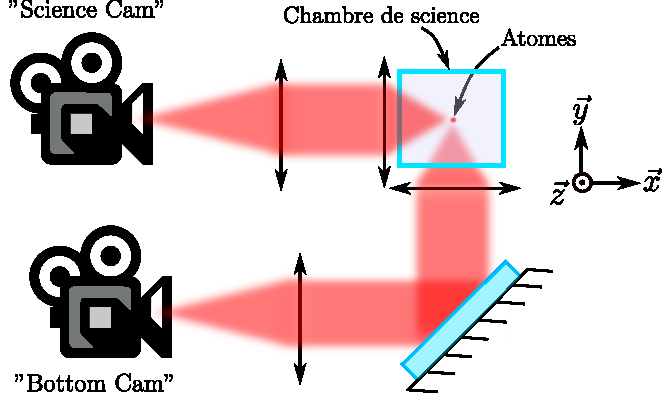
\includegraphics[scale=1]{Fig/BEC_manip/img_science_3.pdf}
\caption{\textbf{Dispositif d'imagerie par fluorescence pour la chambre de science.} Une caméra capte les photons de fluorescence émis par les atomes selon une direction horizontale (\emph{Science Cam}), tandis qu'une autre capte ceux émis vers le bas avec un transport d'image (\emph{Bottom Cam}). Les faisceaux de fluorescence ne sont pas représentés ici (selon l'axe $\vec{z}$).}
\label{fig:img_science}
\end{figure}

L'intensité diffusée captée dans le plan d'imagerie est alors donnée par:
\begin{equation}
I_{\mathrm{fluo}}(y,z)\approx\frac{\Omega}{4\pi} \Gamma_{\mathrm{sp}}\hb \omega_0 n_{\mathrm{2D}}(y,z) \text{ ,}
\label{eq:img_fluo}
\end{equation}
avec $\Omega \simeq \pi \ON^2$ l'angle solide dans lequel les photons de fluorescence sont captés par le système d'imagerie d'ouverture numérique $\ON\sim 0.4$. \\
Théoriquement, une unique image suffit à obtenir le profil de densité atomique. Cependant, une seconde image capturée avec les faisceaux de fluorescence allumés est utilisée afin de soustraire un éventuel bruit dû à ceux-ci. 

%Étant donné le nombre de paramètres non parfaitement connus dans la formule \ref{eq:img_fluo}, il est nécessaire de calibrer cette méthode d'imagerie. La calibration du nombre d'atomes se fait par comparaison avec l'imagerie par absorption. Si la comparaison est directe dans la première chambre, celle de l'imagerie dans la chambre de science est un peu plus délicate. La méthode retenue par l'équipe consiste à calibrer l'efficacité du transfert par la pince optique à l'aide d'allers-retours pour déterminer le nombre d'atomes attendu dans la seconde chambre.


